\subsection{Gradient decent methods}

\begin{figure}[H]
\centering
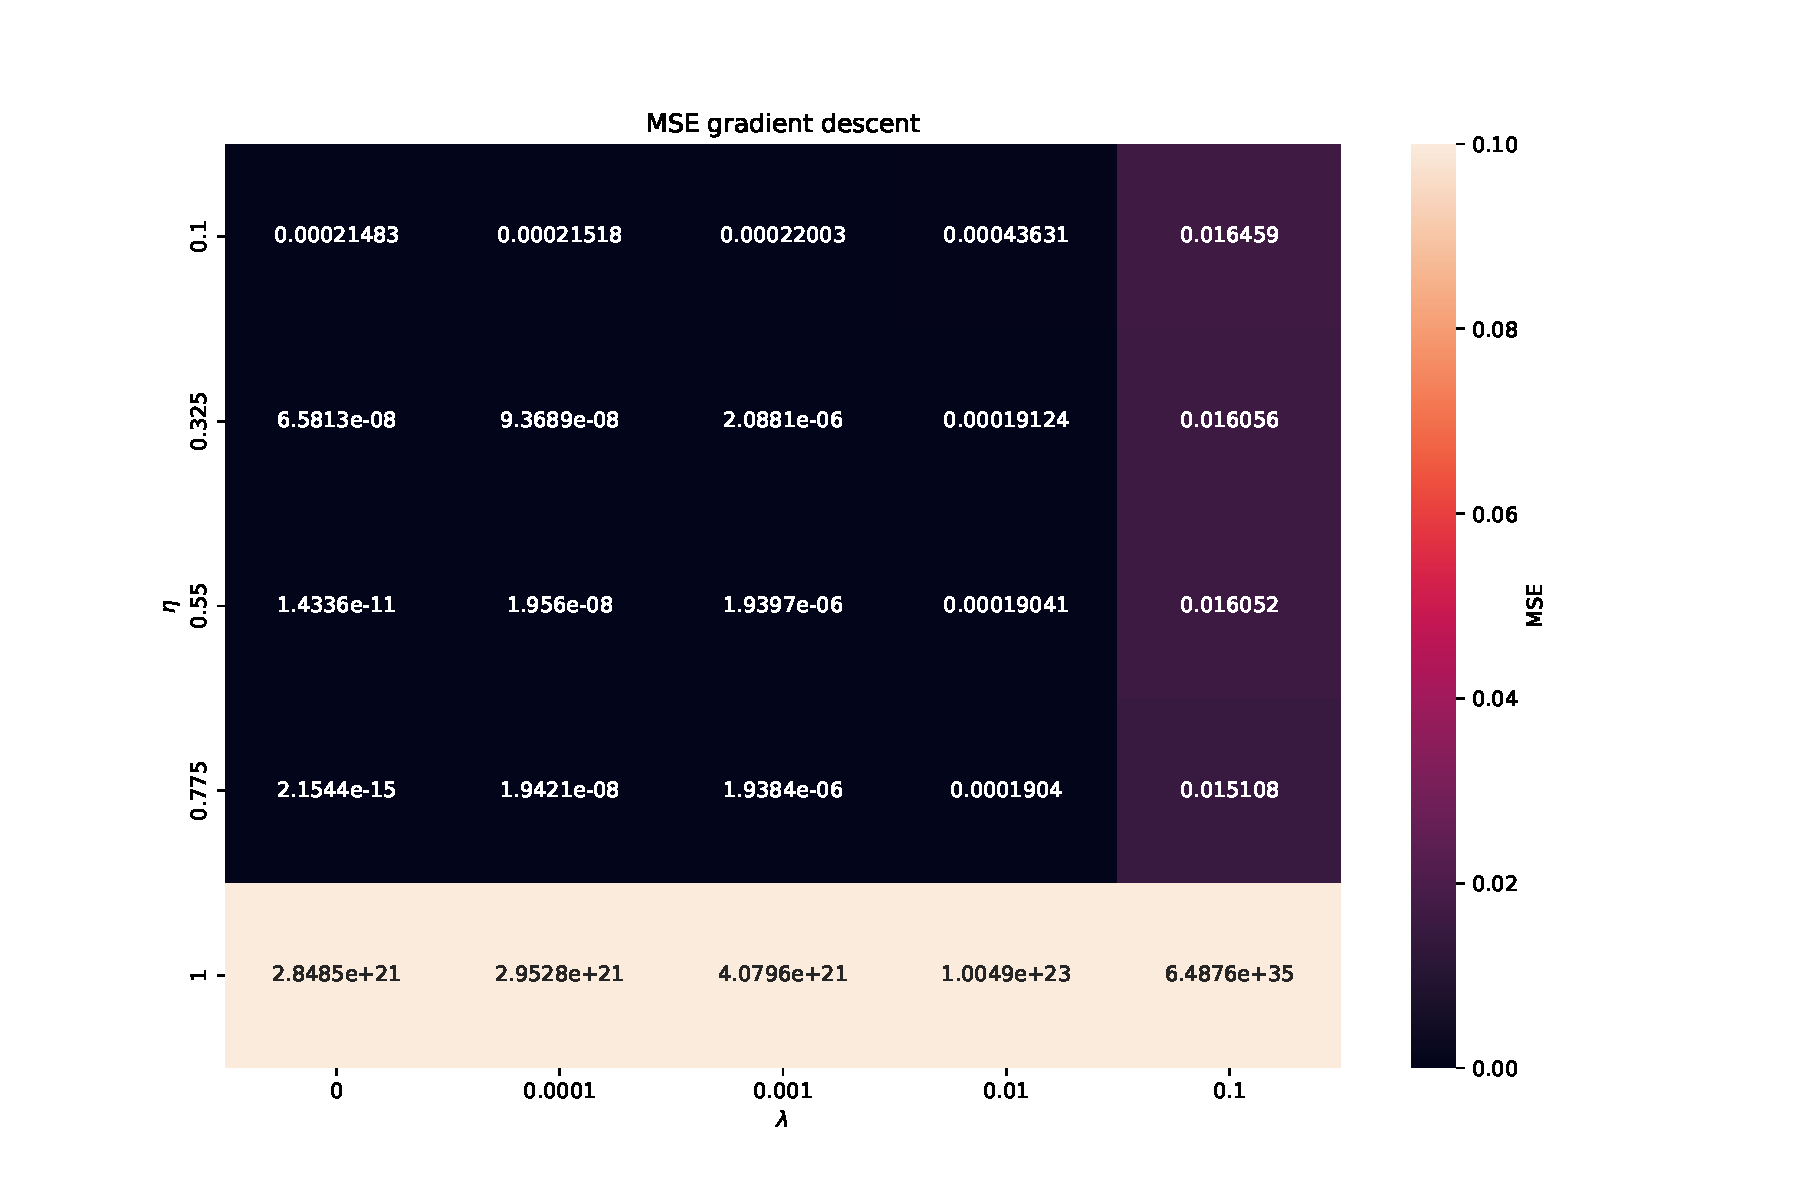
\includegraphics[width=0.8\textwidth]{Figures/PartA/gd_MSE(eta,lmb)}
\caption{Plain gradient descent: test MSE as a function of \(\eta \) and \(\lambda \). 
The parameters utilized are shown in table \ref{tab:GD_parameters_run_1_2} under run 1.}
\label{fig:gd_MSE-eta-lmb-}
\end{figure}

\begin{figure}[H]
\centering
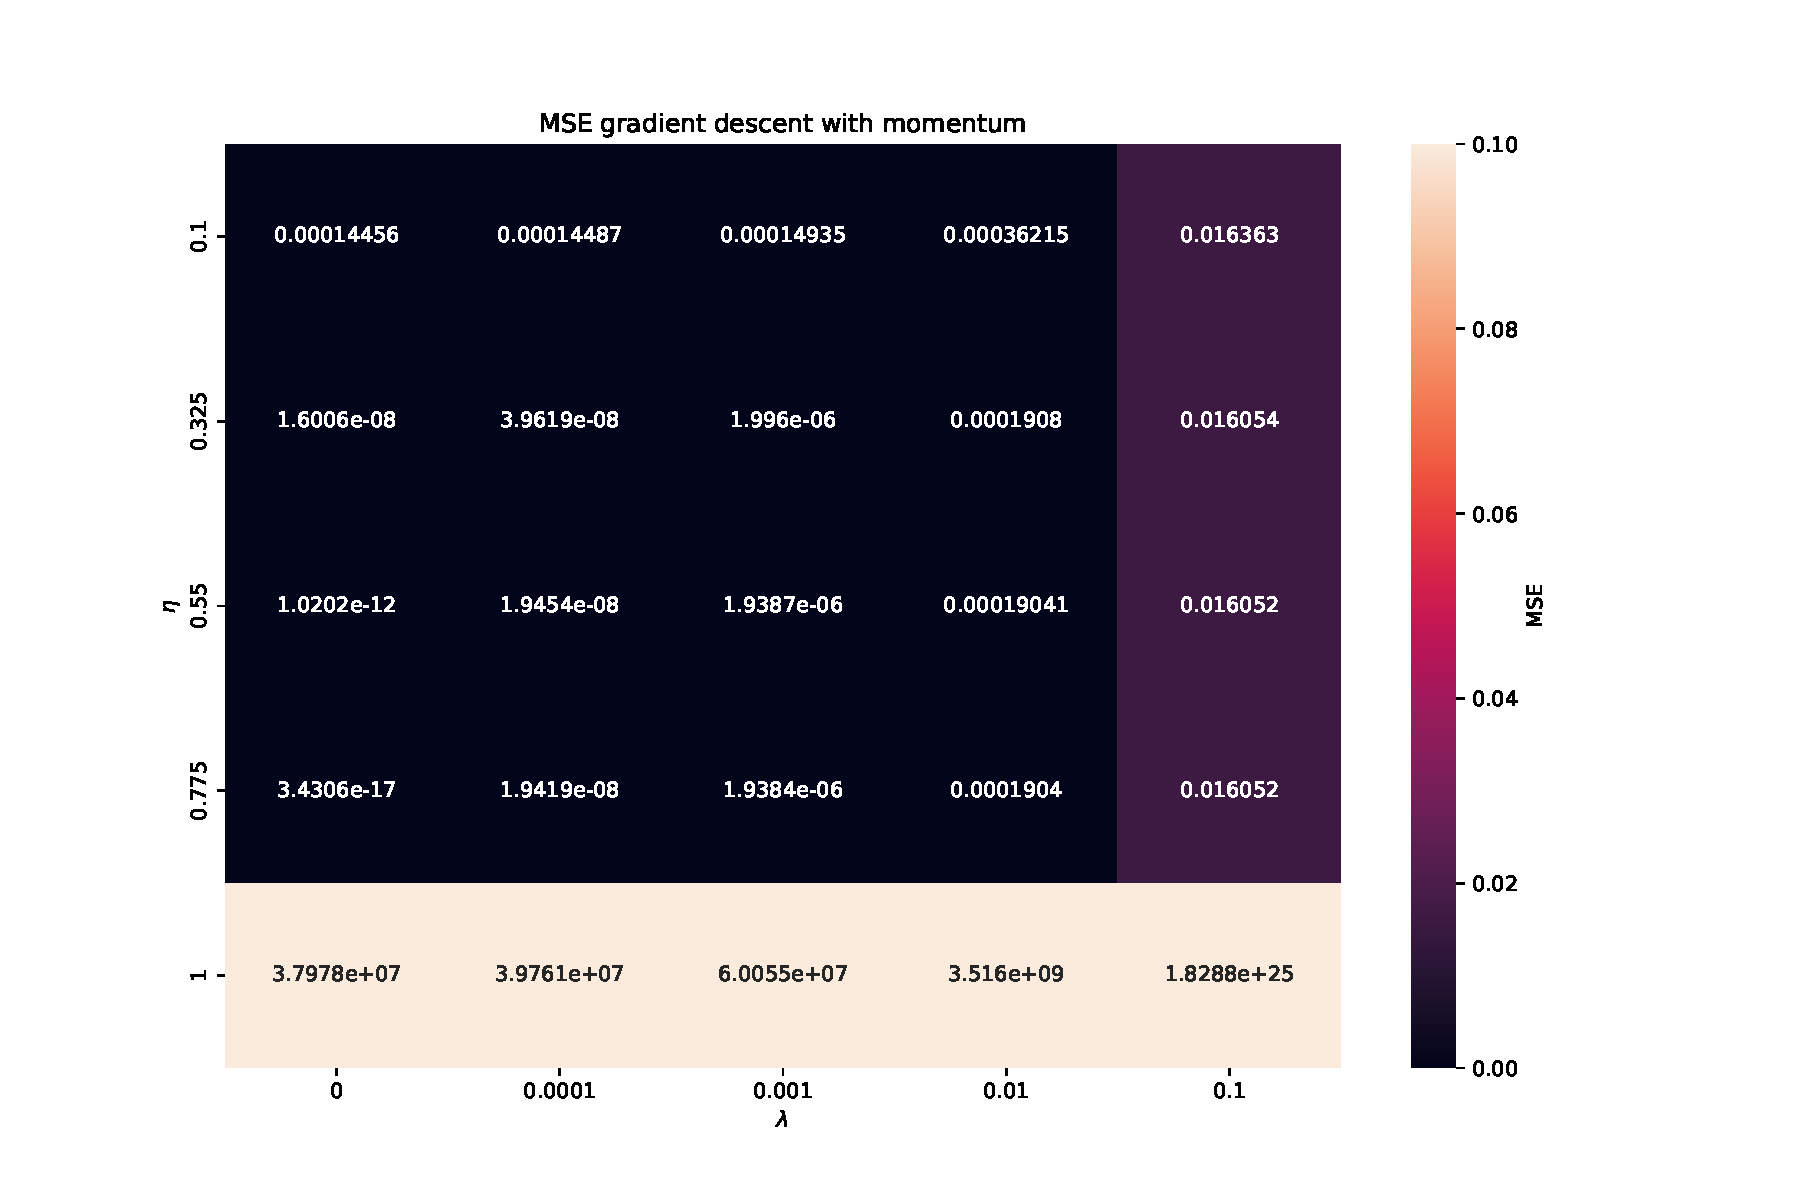
\includegraphics[width=0.8\textwidth]{Figures/PartA/gdm_MSE(eta,lmb)}
\caption{Gradient descent with momentum: test MSE as a function of \(\eta \) and \(\lambda \).
 The parameters utilized are shown in table \ref{tab:GD_parameters_run_1_2} under run 1.}
\label{fig:gdm_MSE-eta-lmb-}
\end{figure}

\begin{figure}[H]
\centering
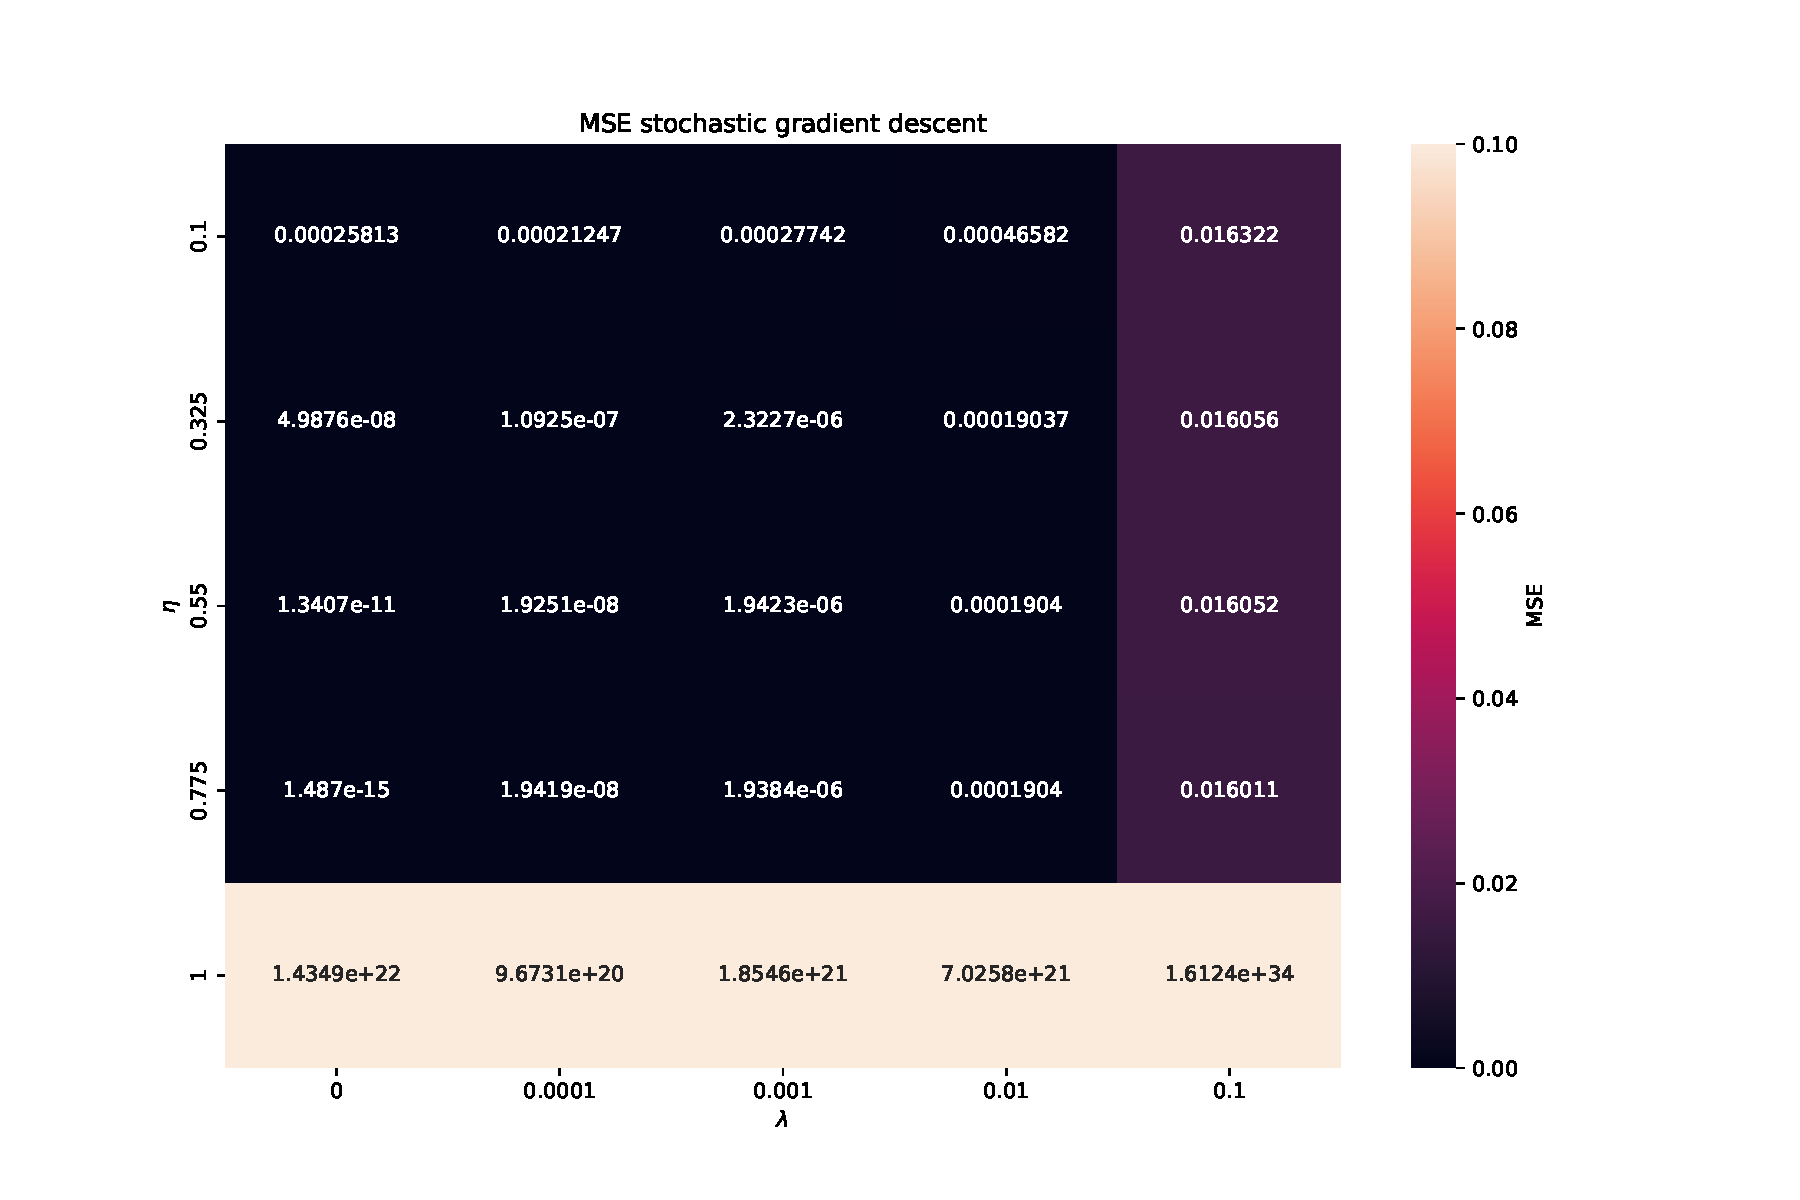
\includegraphics[width=0.8\textwidth]{Figures/PartA/sgd_MSE(eta,lmb)}
\caption{Plain stochastic gradient descent: test MSE as a function of \(\eta \) and \(\lambda \).
 The parameters utilized are shown in table \ref{tab:GD_parameters_run_1_2} under run 1.}
\label{fig:sgd_MSE-eta-lmb-}
\end{figure}

\begin{figure}[H]
\centering
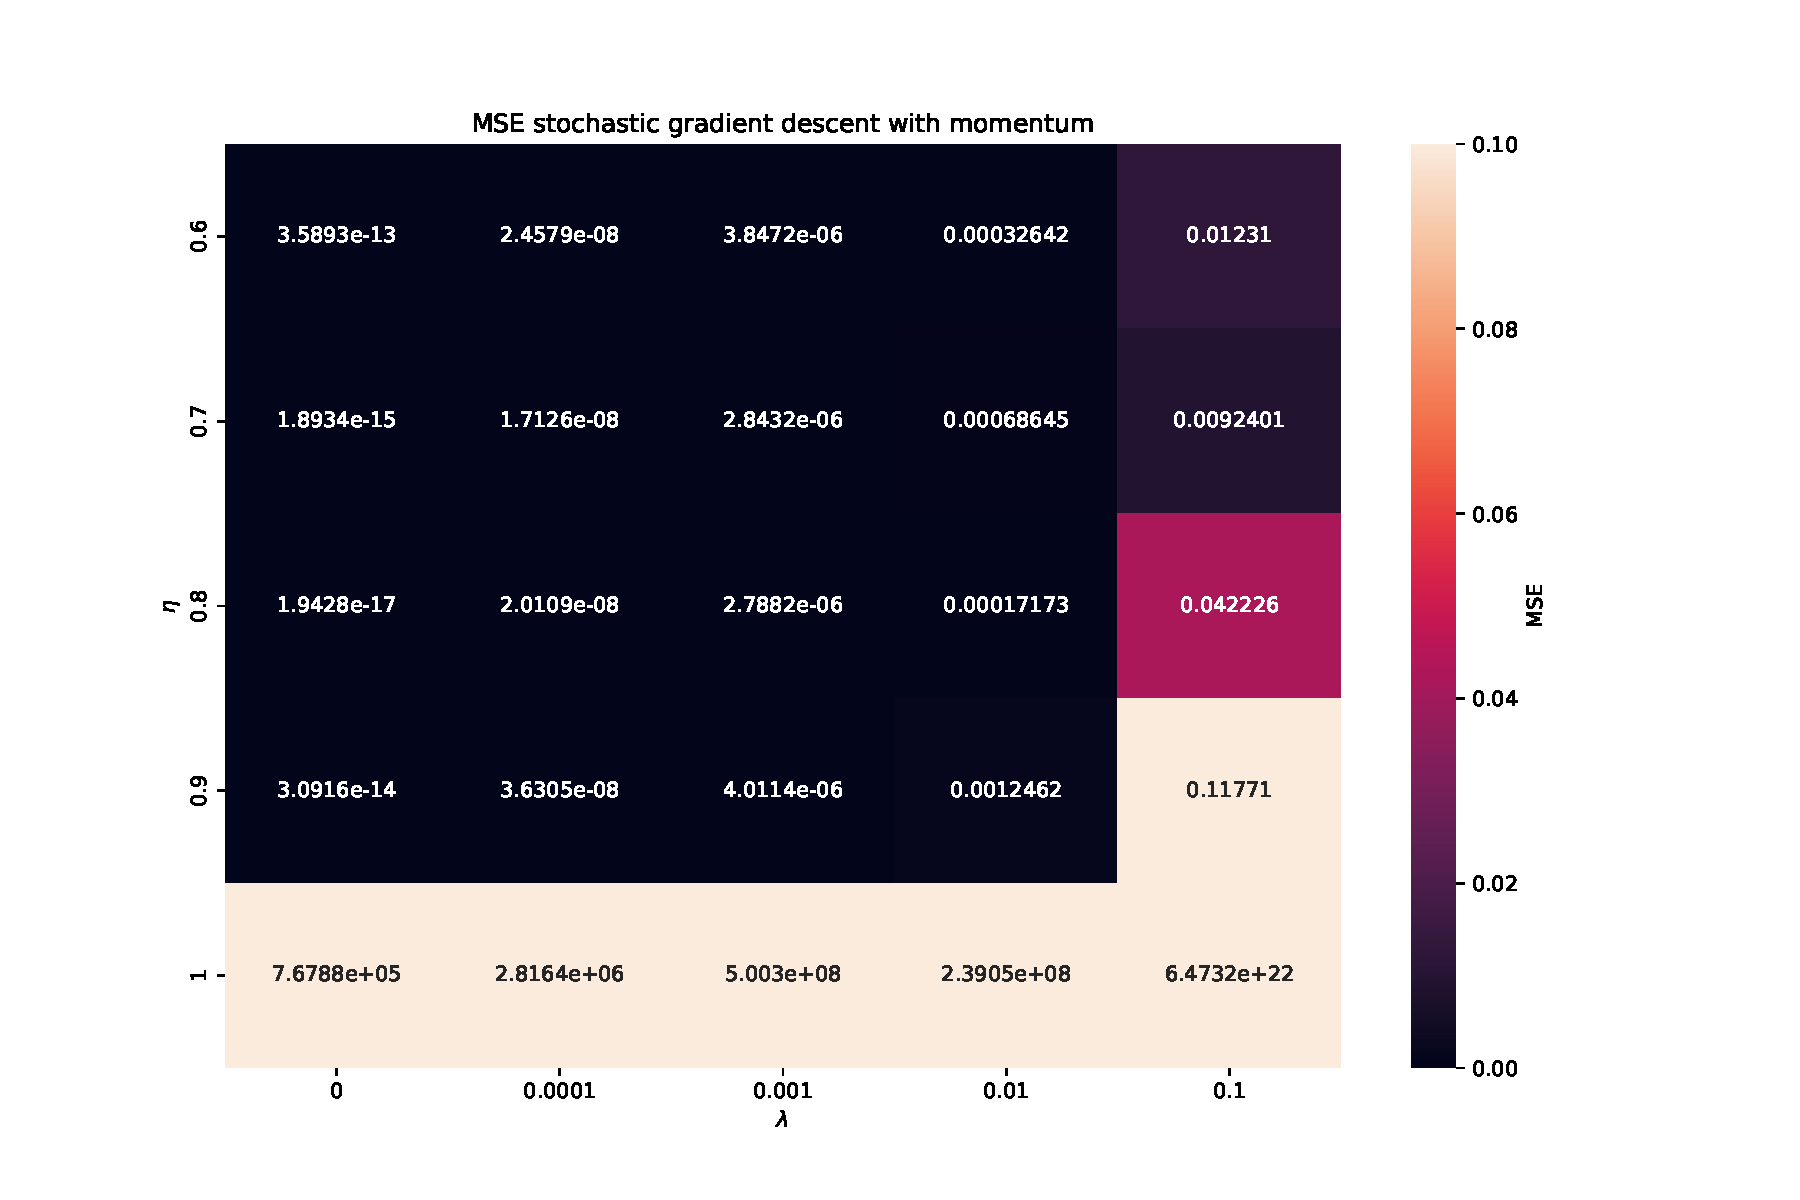
\includegraphics[width=0.8\textwidth]{Figures/PartA/sgdm_MSE(eta,lmb)}
\caption{Stochastic gradient descent with momentum: test MSE as a function of \(\eta \) and \(\lambda \).
 The parameters utilized are shown in table \ref{tab:GD_parameters_run_1_2} under run 1.}
\label{fig:sgdm_MSE-eta-lmb-}
\end{figure}

Figure \ref{fig:gd_MSE-eta-lmb-}-\ref{fig:sgdm_MSE-eta-lmb-} shows MSE scores of the test data for 
plain and stochastic gradient descent with and without momentum as a function of
different learning rates \(\eta \) and L2-regularzation parameters \(\lambda \). Both plain and 
stochastic gradient descent has the same amount of total iterations as there are $25$ sgd epochs 
and $n\_data/mini\_batch\_size=80/20=4$ minibatches giving a total amount of $25 \cdot 4 = 100$ 
iterations for stochastic gradient descent. We observe that we get a better MSE score with larger 
learning rates up to a point where the score blows up shown for $\eta=1$. This makes sense as larger 
learning rates results in larger update to the parameters $\bf{\theta } $. Thus, too large learning reate 
will overshoot the minima of the cost function, while too small will cause slow convergence.  
We also observe the MSE to increase with increasing L2-regularzation parameter $\lambda $. This also 
makes sense as $\lambda $ counters overfitting at the cost of poorer training fit, but since we are 
optimizing the coefficients of a same order polynomial as the target, overfitting will not be a problem.
We are therefore better off without the L2-regularzation parameter. 

The momentum 
term is proportional to the previous variable change, such that when overshooting, this vector term will be in the 
(somewhat) opposite direction and thus causing less of a step wich is why we observe the MSE blowing up without momentum,
while not blowing up with momentum for $\eta =0.9$. Momentum also gives better scores as it allows for bigger steps
before the minima of the cost function is traversed. 

The performance of plain and stochastic gradient descent is similar, with plain being slightly better. As the 
cost functions are convex, there is no local minimas for plain gradient descent to get stuck on, such that the 
performance difference will come down to the randomly sampled minibatches in stochastic gradient descent. 



\begin{figure}[H]
\centering
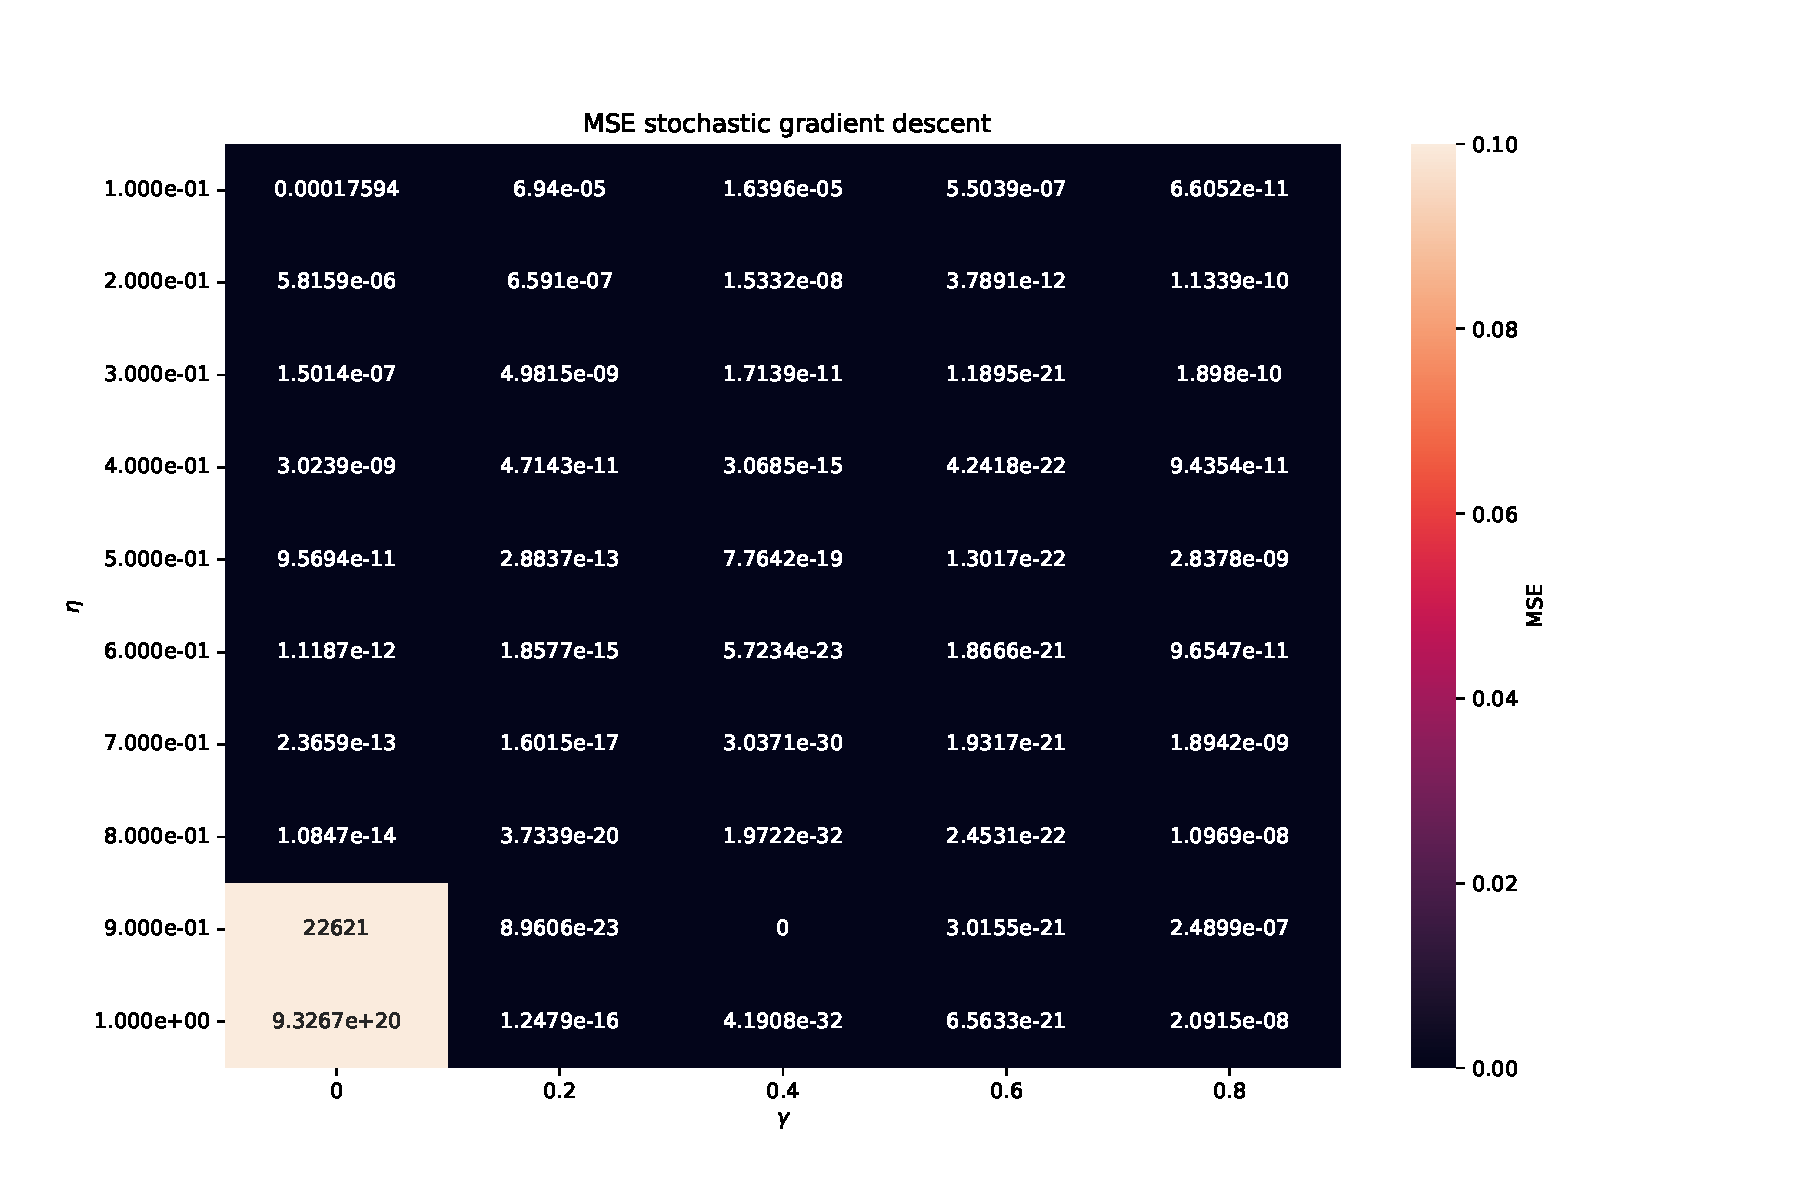
\includegraphics[width=0.8\textwidth]{Figures/PartA/_sgdm_MSE(eta,momentum)}
\caption{Stochastic gradient descent: MSE as a function of momentum parameter $\gamma$  and \(\eta \)	 }
\label{fig:_sgdm_MSE-eta-momentum-}
\end{figure}

\begin{figure}[H]
\centering
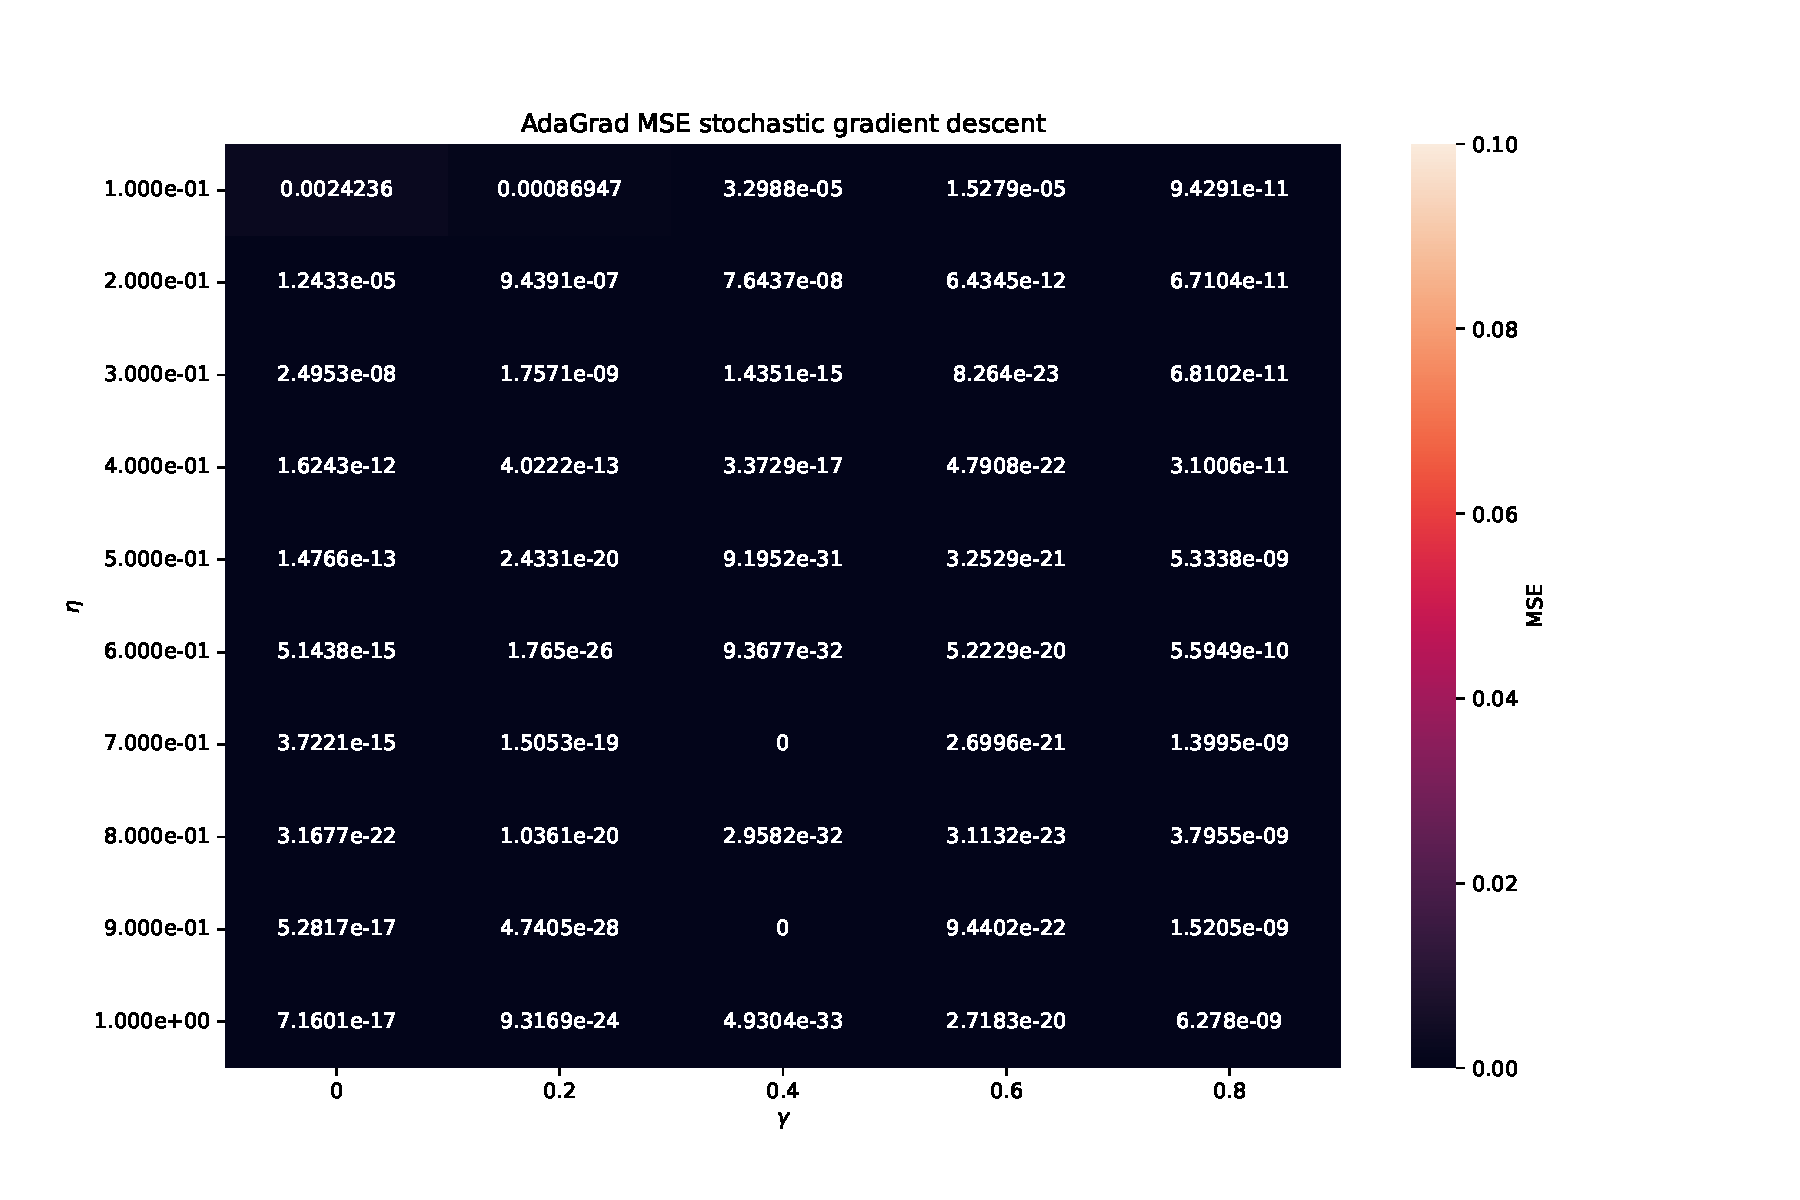
\includegraphics[width=0.8\textwidth]{Figures/PartA/AdaGrad_sgdm_MSE(eta,momentum)}
\caption{Stochastic gradient descent, with momentum and tuning method AdaGrad: MSE as a function of momentum parameter $\gamma$ and \(\eta \)	 }
\label{fig:AdaGrad_sgdm_MSE-eta-momentum-}
\end{figure}

\begin{figure}[H]
\centering
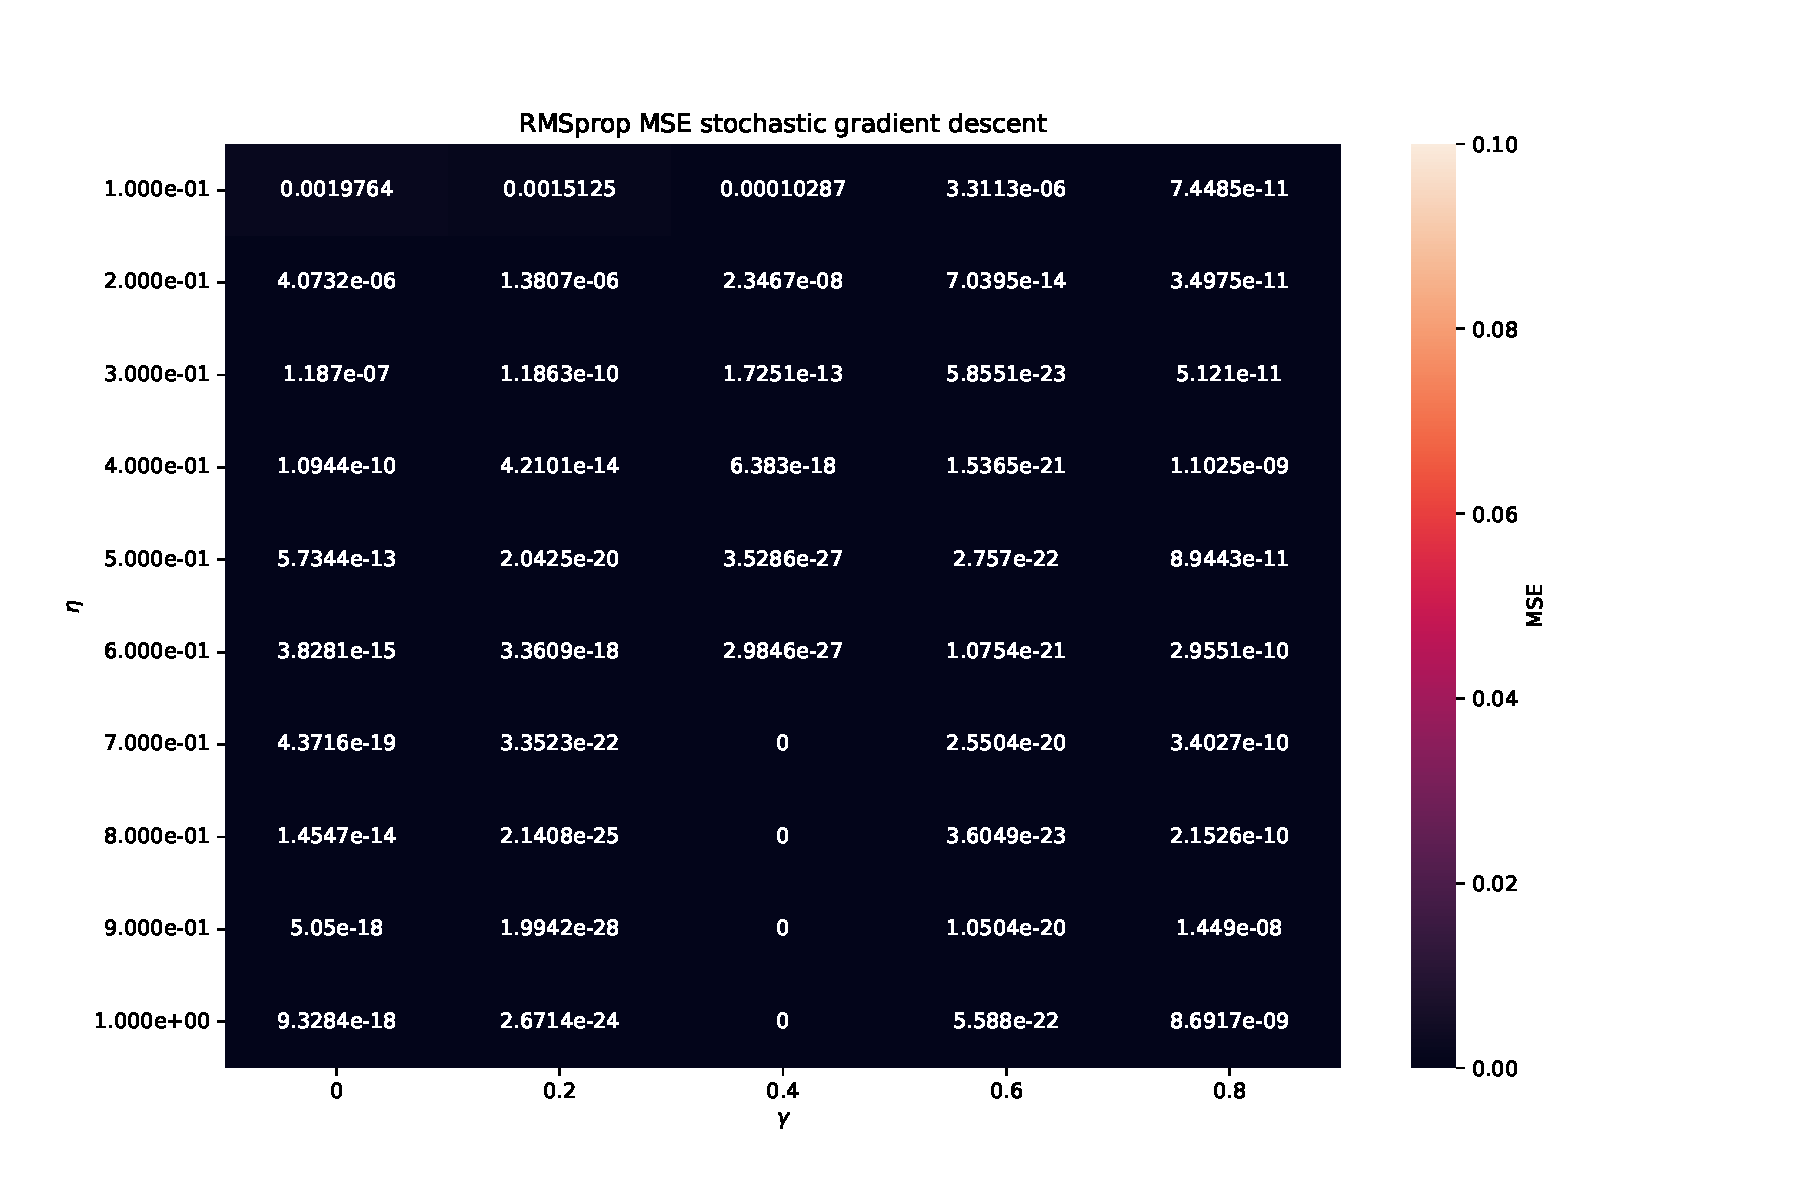
\includegraphics[width=0.8\textwidth]{Figures/PartA/RMSprop_sgdm_MSE(eta,momentum)}
\caption{Stochastic gradient descent, with momentum and tuning method RMS\_prop: MSE as a function of momentum parameter $\gamma$ and \(\eta \)	 }
\label{fig:RMSprop_sgdm_MSE-eta-momentum-}
\end{figure}

\begin{figure}[H]
\centering
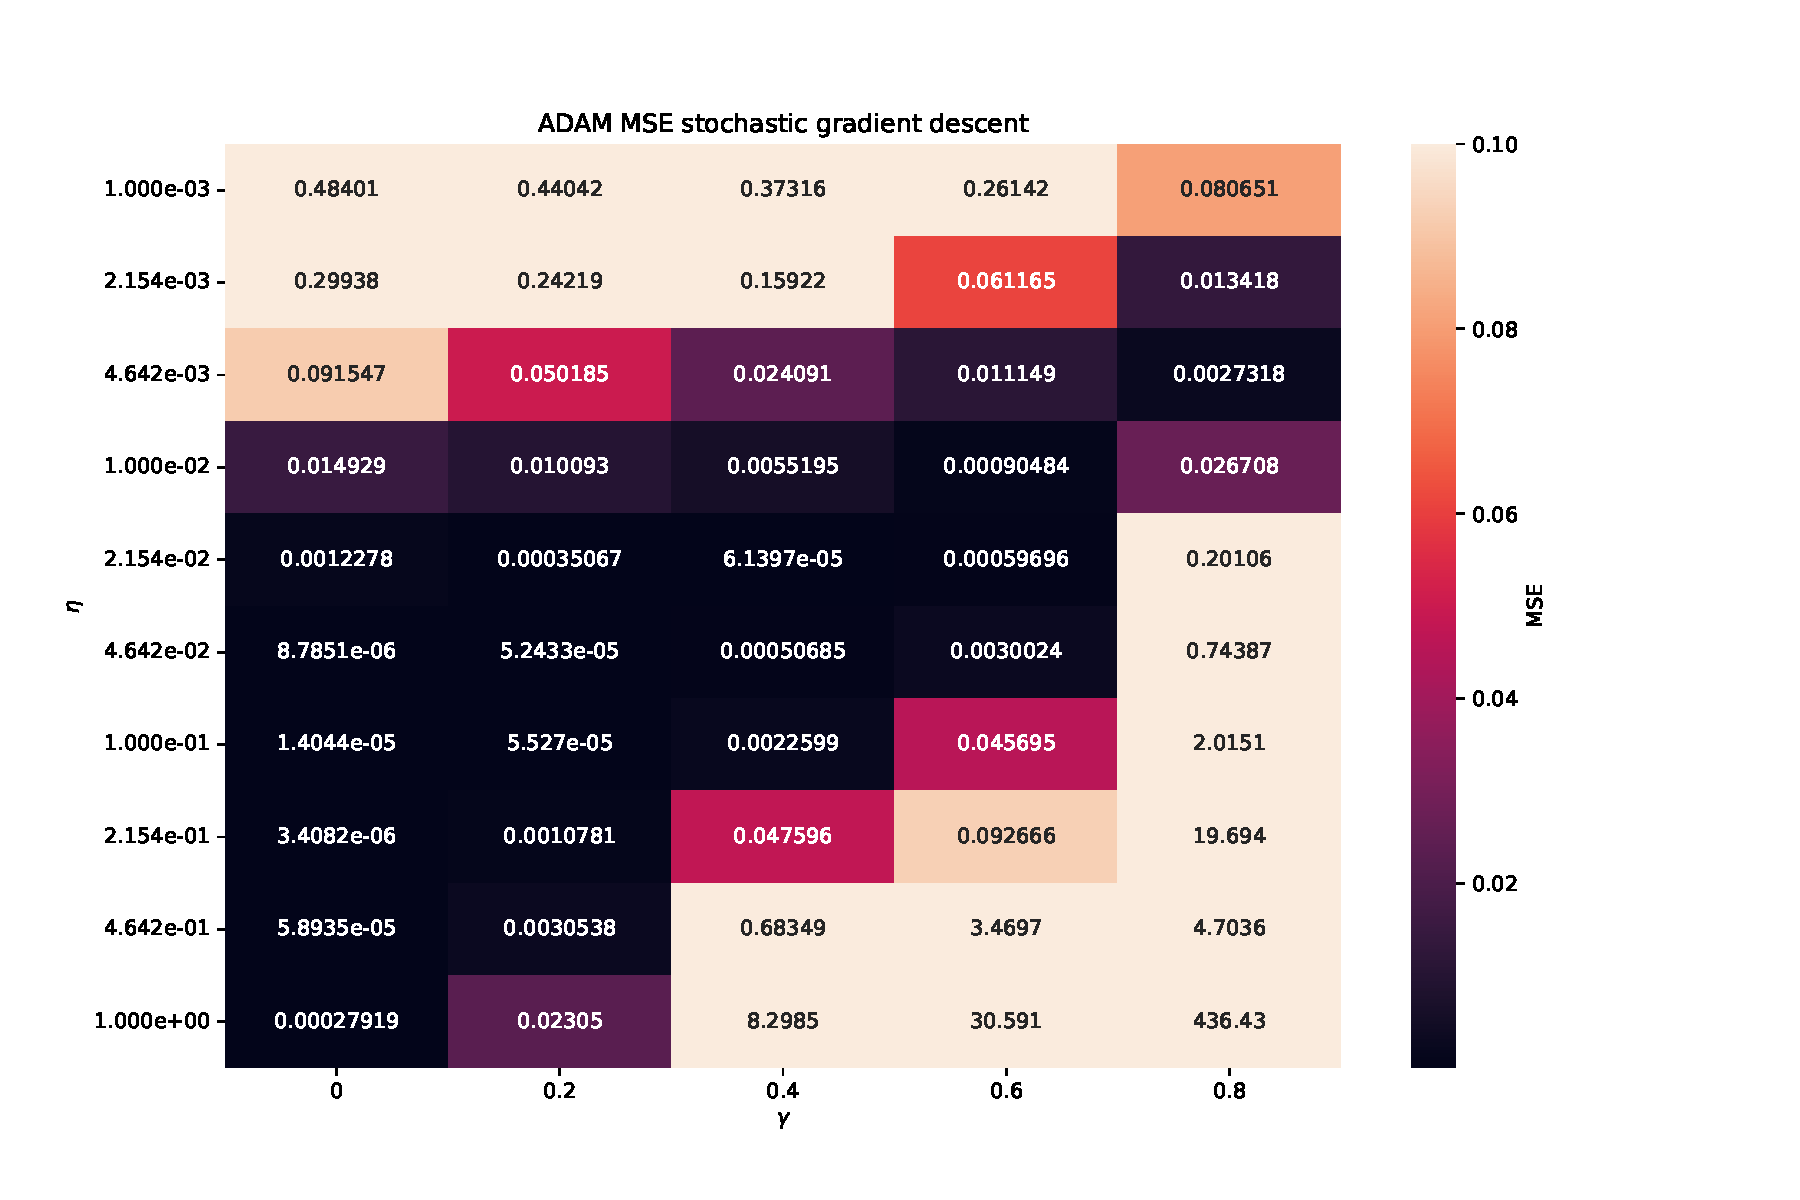
\includegraphics[width=0.8\textwidth]{Figures/PartA/ADAM_sgdm_MSE(eta,momentum)}
\caption{Stochastic gradient descent, with momentum and tuning method ADAM: MSE as a function of momentum parameter $\gamma$ and \(\eta \)	 }
\label{fig:ADAM_sgdm_MSE-eta-momentum-}
\end{figure}

Figure \ref{fig:_sgdm_MSE-eta-momentum-}-\ref{fig:ADAM_sgdm_MSE-eta-momentum-}, shows the MSE from stochastic gradient descent for different
learning rates $\eta $ and momentum parameters $\gamma $ for no tuning method, AdaGrad, RMSprop and ADAM. We observe that ADAM does not benefit 
from momentum, while AdaGrad, RMSprop, and plain stochastic gradient descent shows best results for momentum parameter $\gamma =0.4$ with appropriate 
learning rates $\eta $.  



\begin{figure}[H]
\centering
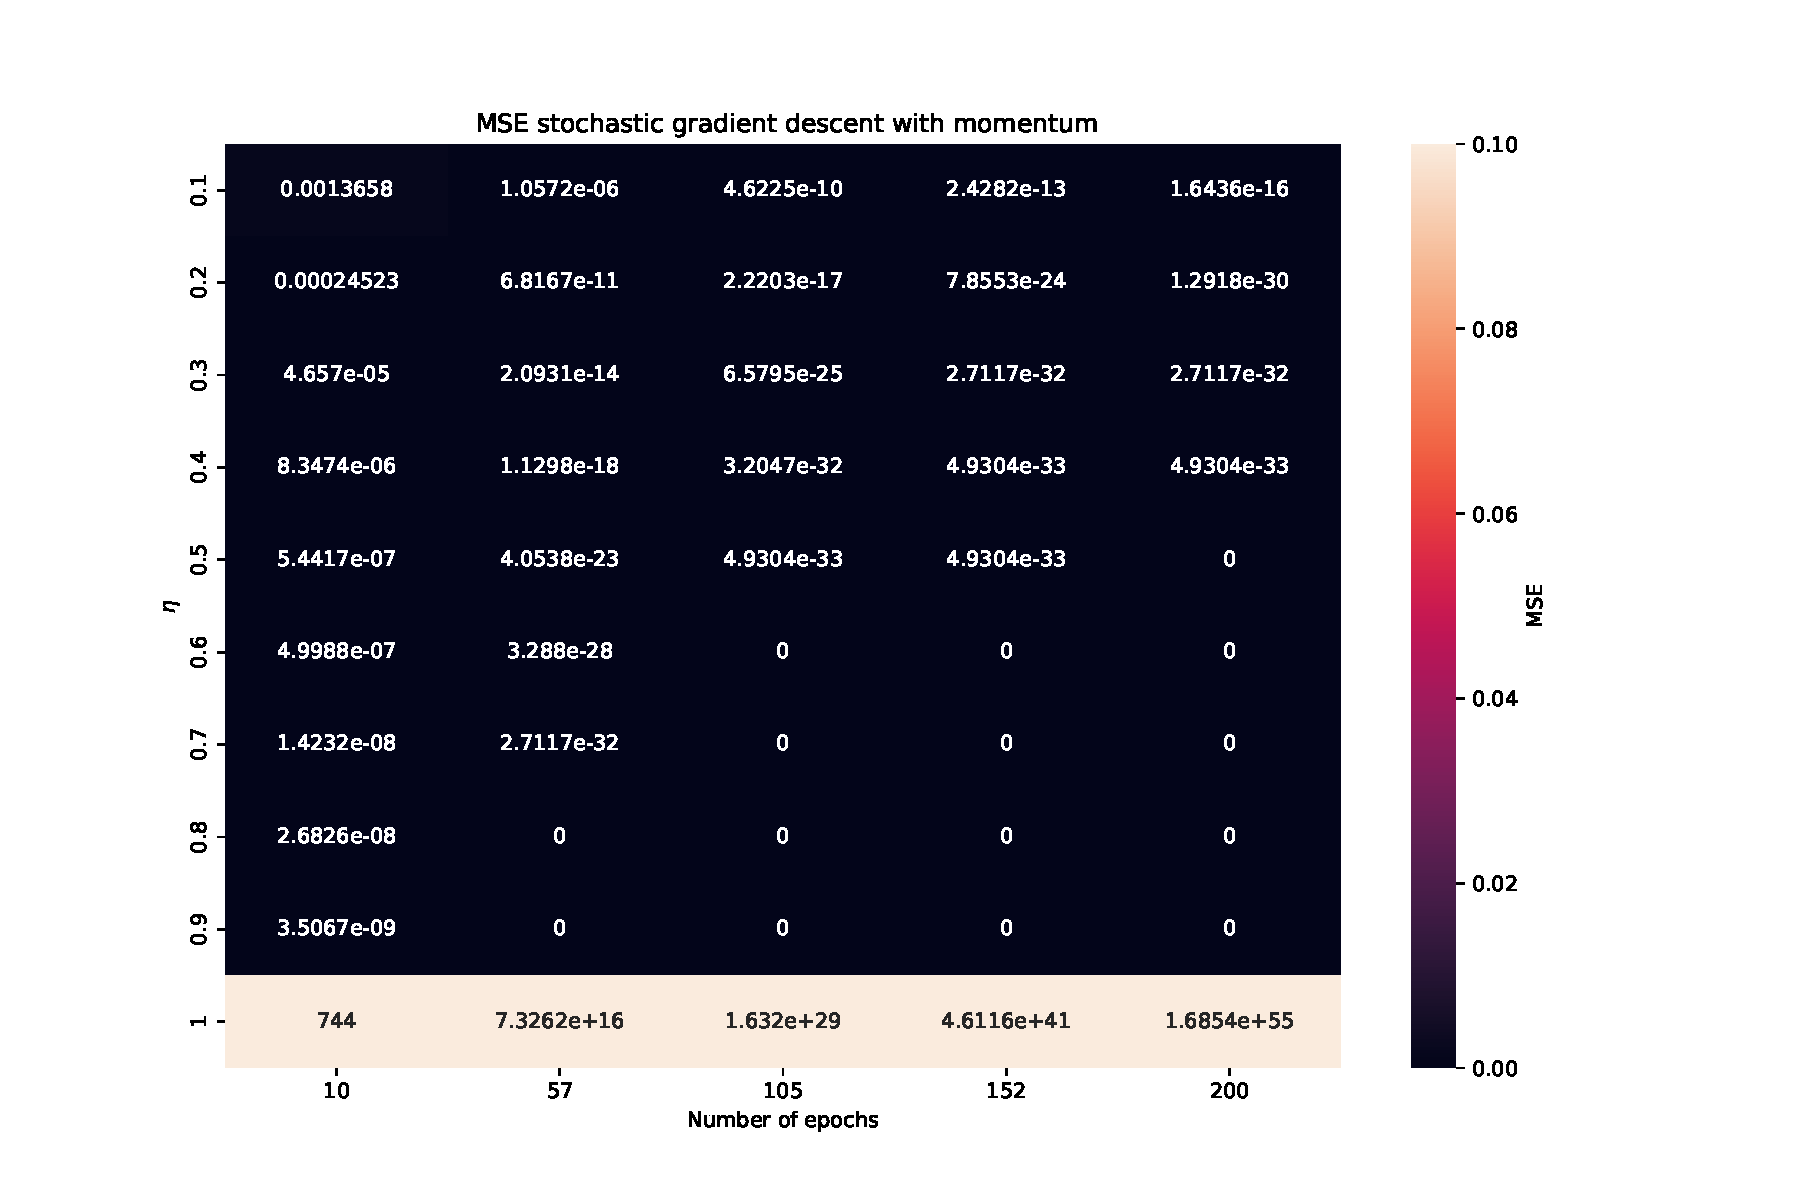
\includegraphics[width=0.8\textwidth]{Figures/PartA/_sgdm_MSE(eta,epochs)}
\caption{Stochastic gradient descent with momentum MSE as a function of epoch number and \(\eta \)	 }
\label{fig:_sgdm_MSE-eta-epochs-}
\end{figure}

\begin{figure}[H]
\centering
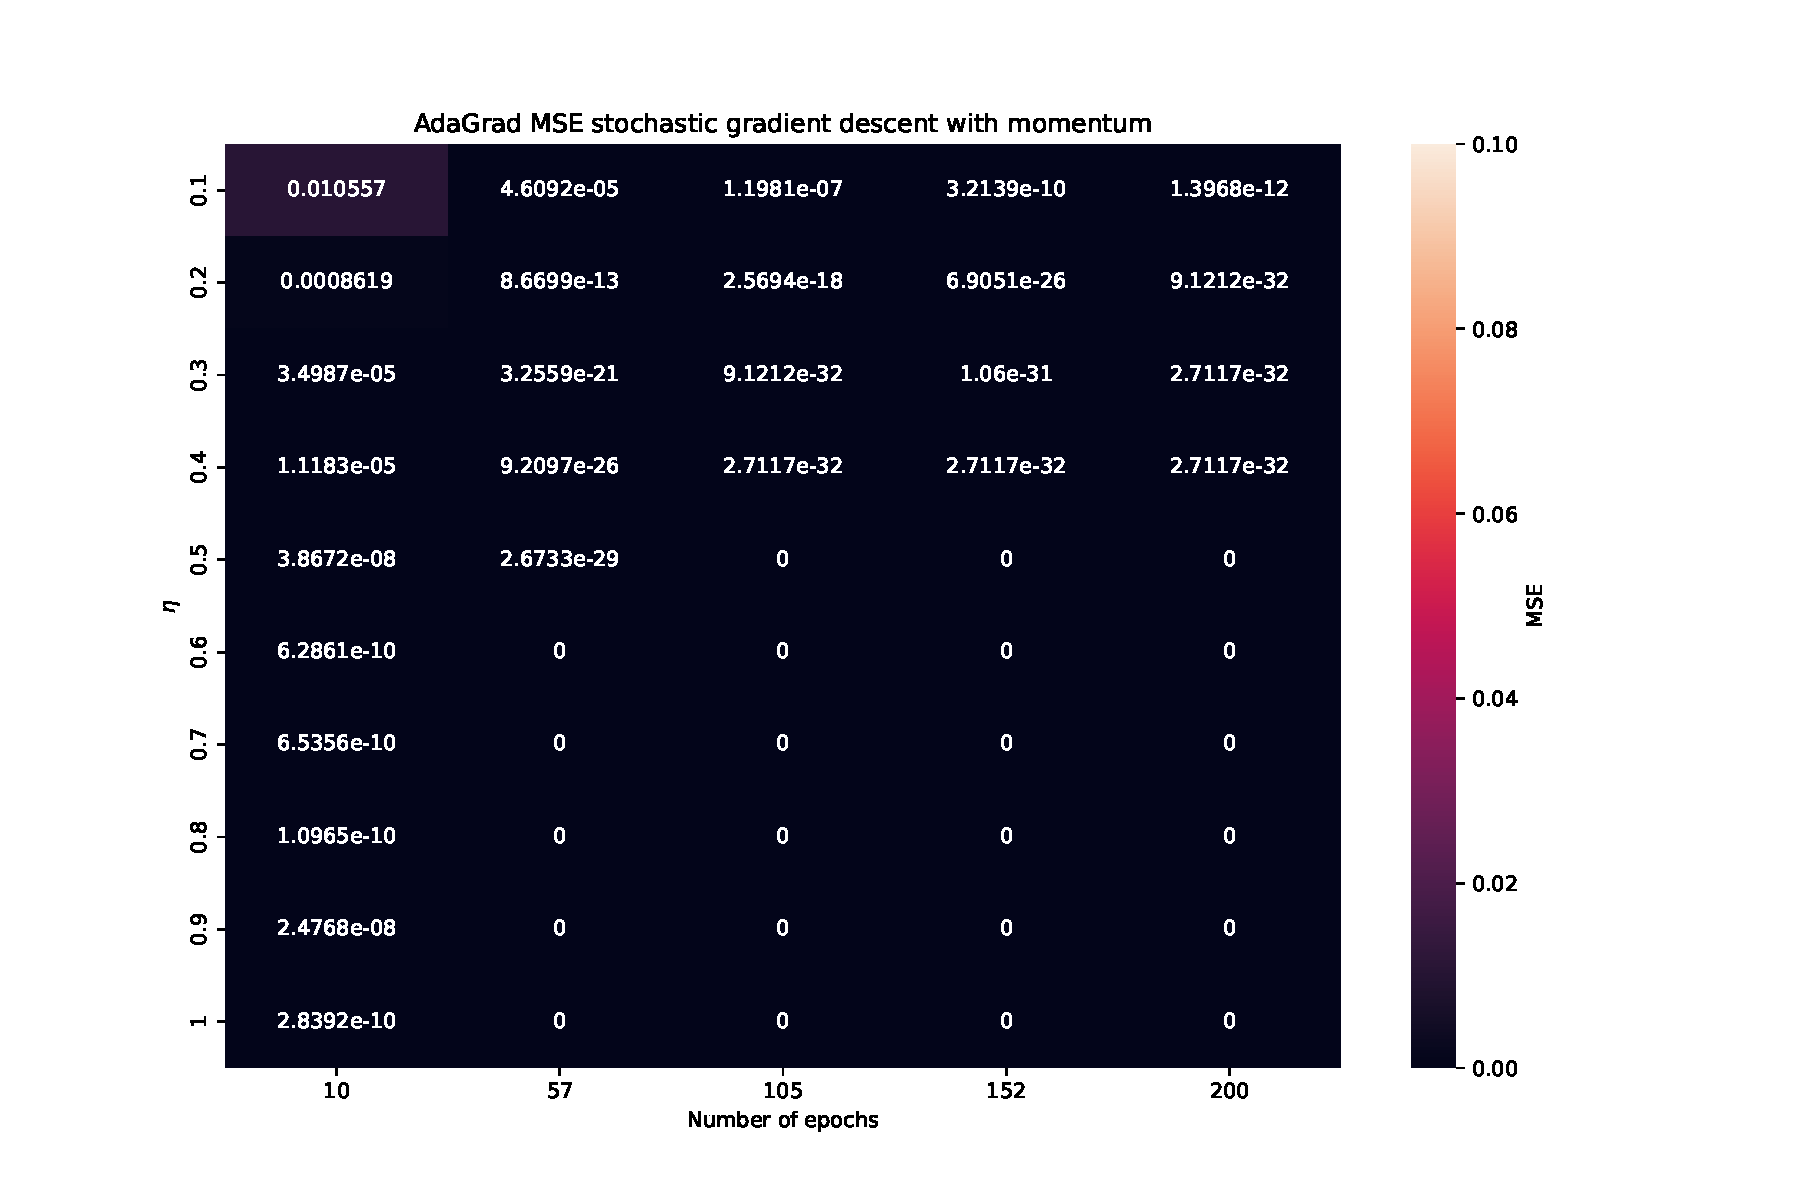
\includegraphics[width=0.8\textwidth]{Figures/PartA/AdaGrad_sgdm_MSE(eta,epochs)}
\caption{Stochastic gradient descent, with momentum and tuning method AdaGrad, MSE as a function of epoch number and \(\eta \)	 }
\label{fig:AdaGrad_sgdm_MSE-eta-epochs-}
\end{figure}

\begin{figure}[H]
\centering
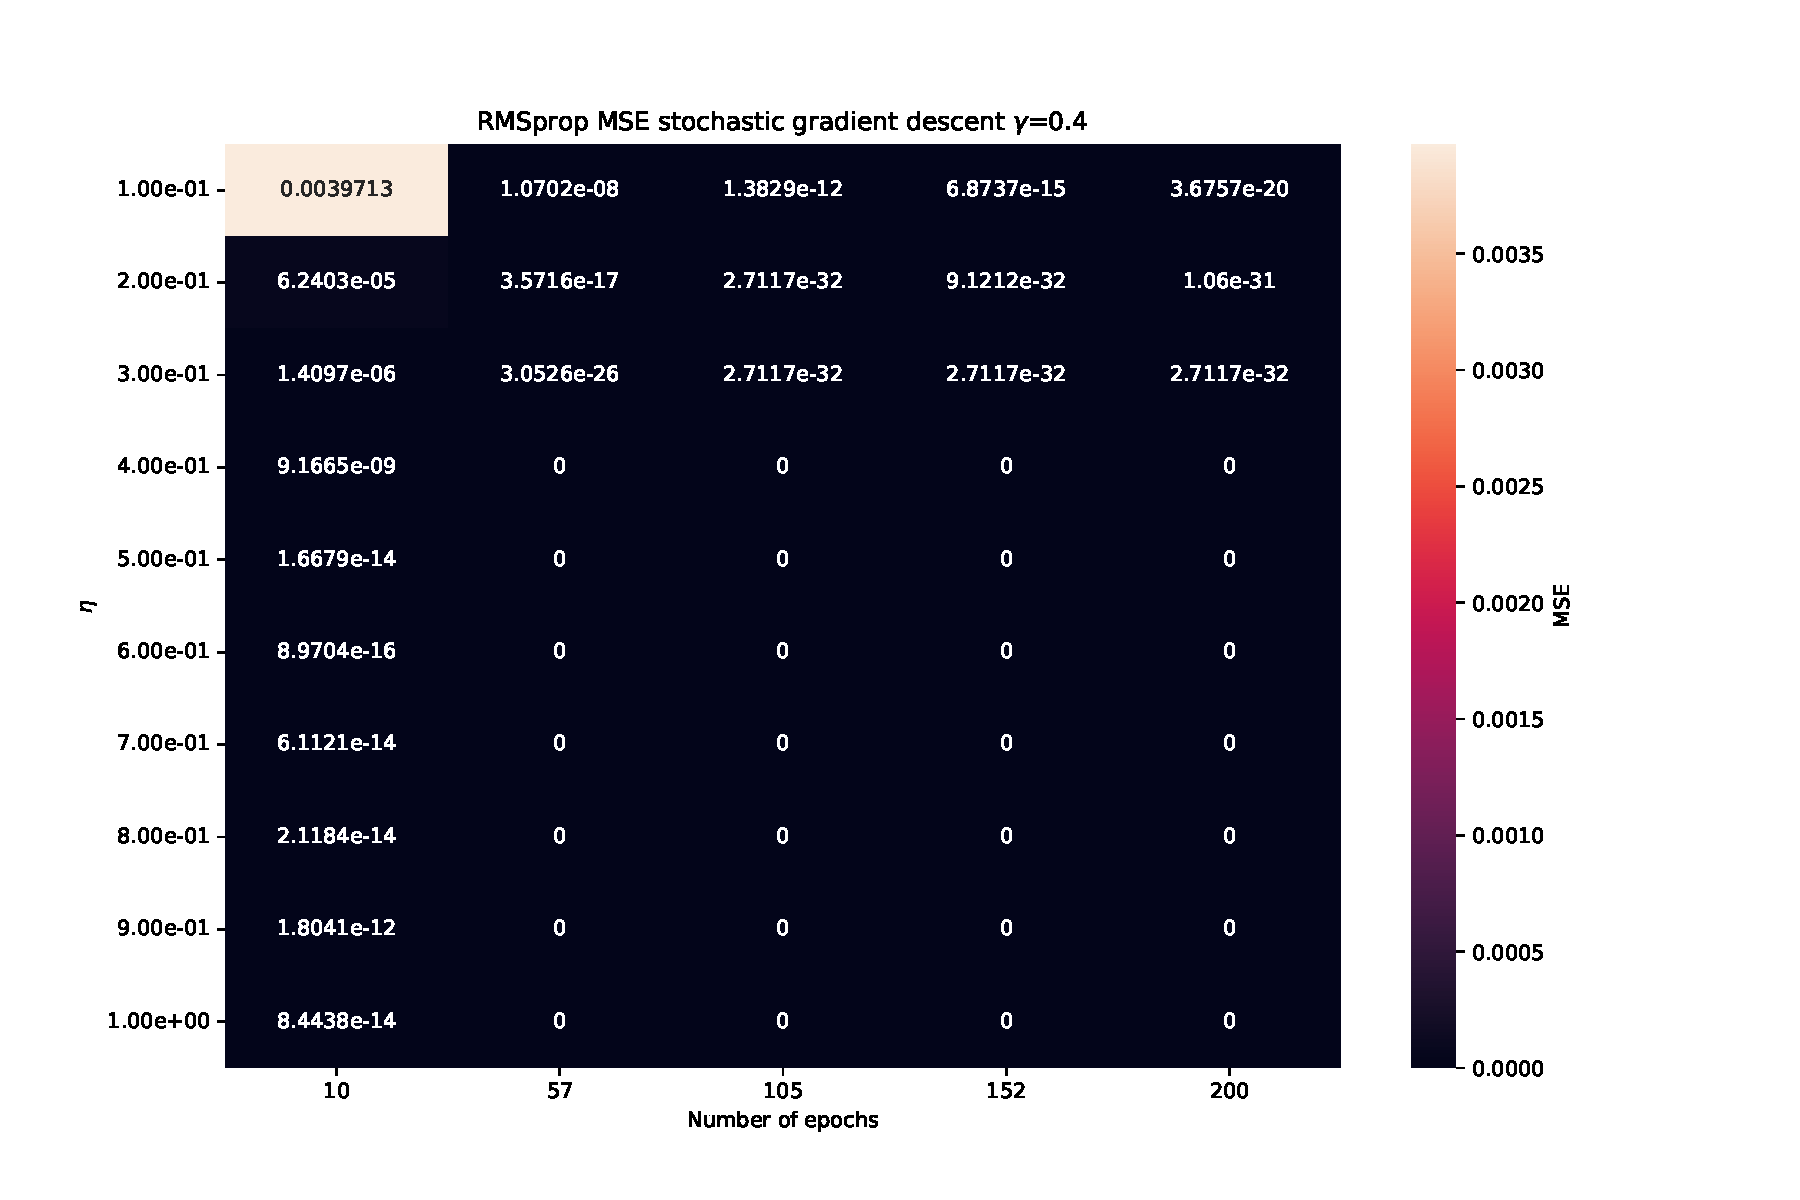
\includegraphics[width=0.8\textwidth]{Figures/PartA/RMSprop_sgdm_MSE(eta,epochs)}
\caption{Stochastic gradient descent, with momentum and tuning method RMS\_prop, MSE as a function of epoch number and \(\eta \)	 }
\label{fig:RMSprop_sgdm_MSE-eta-epochs-}
\end{figure}

\begin{figure}[H]
\centering
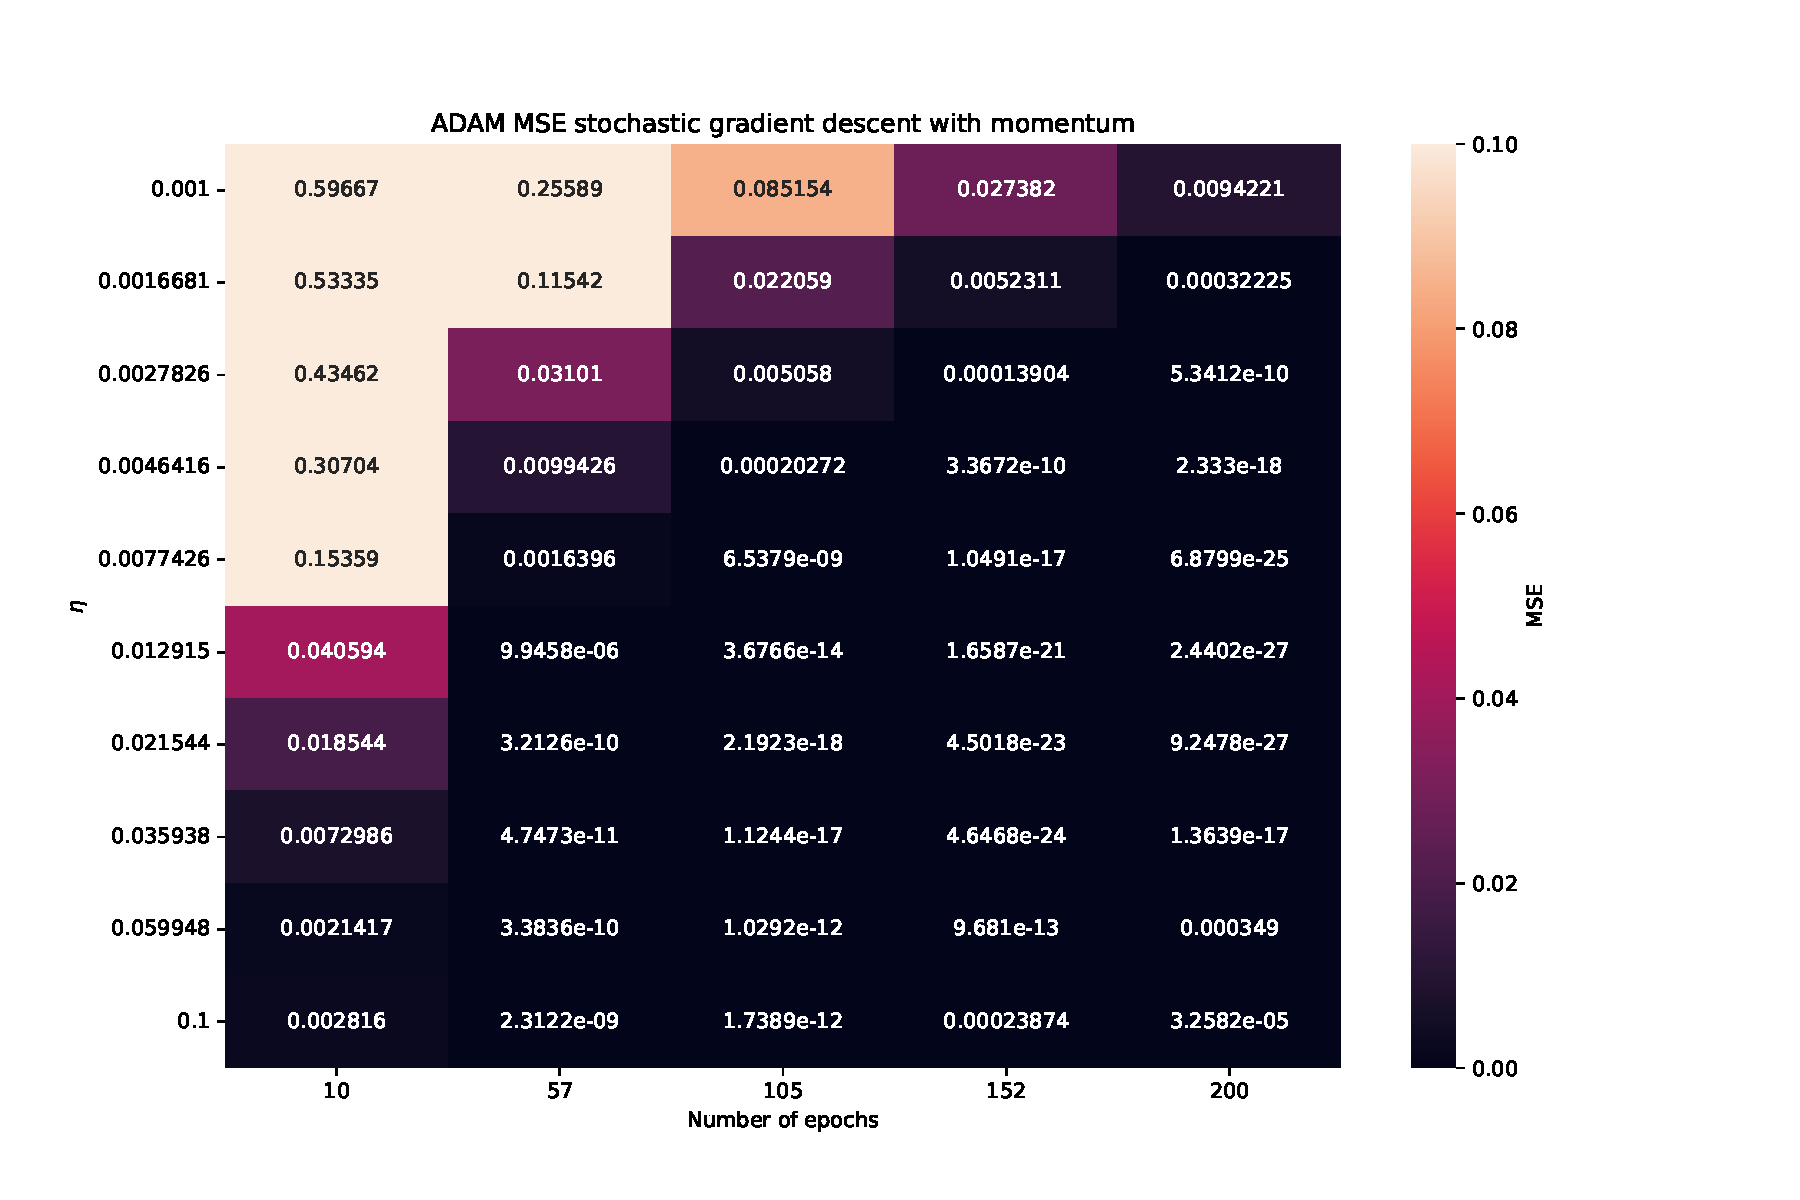
\includegraphics[width=0.8\textwidth]{Figures/PartA/ADAM_sgdm_MSE(eta,epochs)}
\caption{Stochastic gradient descent, with momentum and tuning method ADAM, MSE as a function of epoch number and \(\eta \)	 }
\label{fig:ADAM_sgdm_MSE-eta-epochs-}
\end{figure}



\begin{figure}[H]
\centering
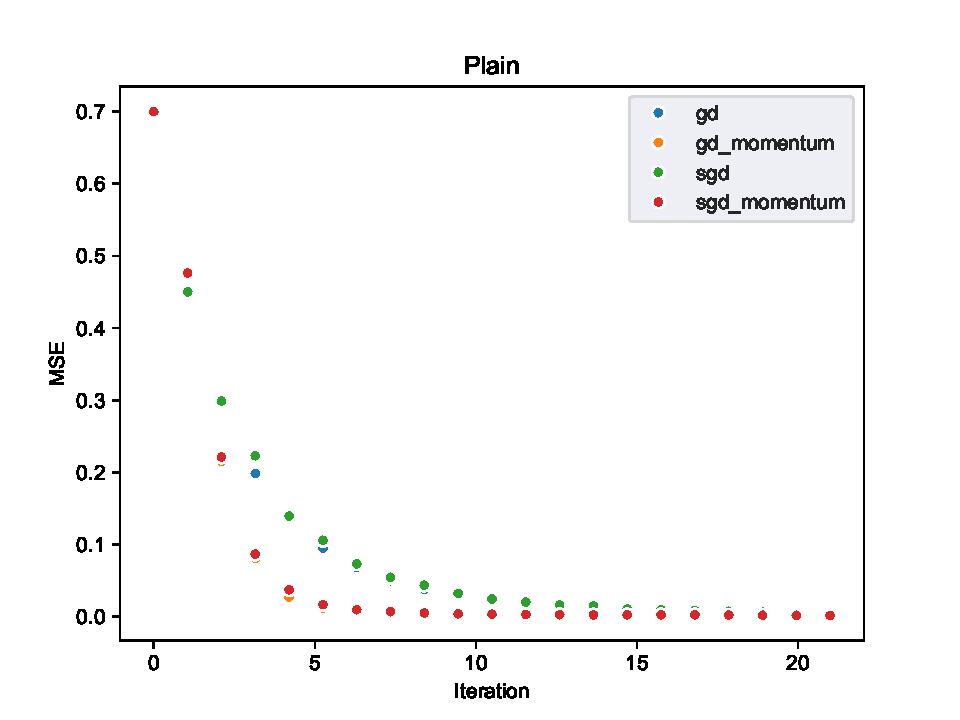
\includegraphics[width=0.8\textwidth]{Figures/PartA/PlainMSE(iter).pdf}
\caption{MSE as a function of iterations for plain and stochastic gradient descent with and without momentum}
\label{fig:PlainMSE-iter-pdf}
\end{figure}

\begin{figure}[H]
\centering
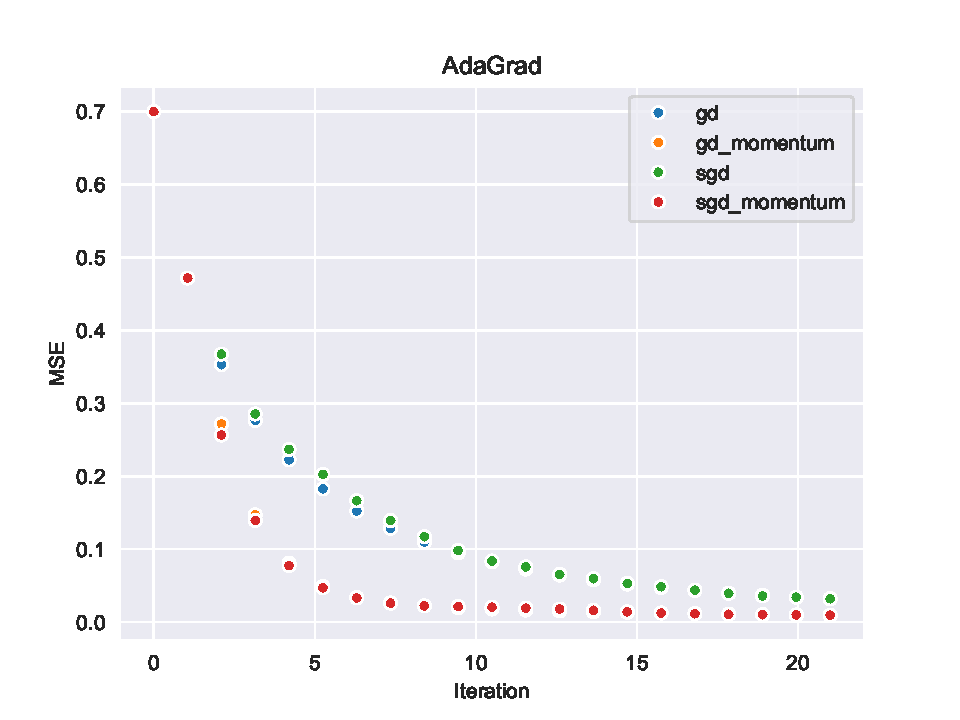
\includegraphics[width=0.8\textwidth]{Figures/PartA/AdaGradMSE(iter).pdf}
\caption{MSE as a function of iterations using tuning method AdaGrad for plain and stochastic gradient descent with and without momentum}
\label{fig:AdaGradMSE-iter-pdf}
\end{figure}

\begin{figure}[H]
\centering
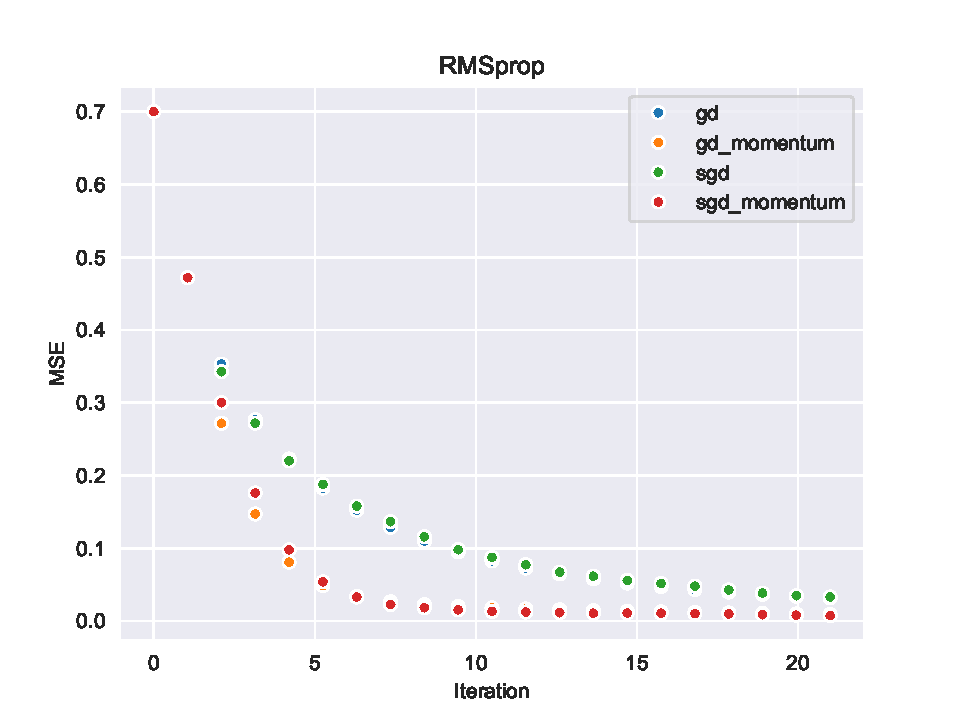
\includegraphics[width=0.8\textwidth]{Figures/PartA/RMSpropMSE(iter).pdf}
\caption{MSE as a function of iterations using tuning method RMSprop for plain and stochastic gradient descent with and without momentum}
\label{fig:RMSpropMSE-iter-pdf}
\end{figure}

\begin{figure}[H]
\centering
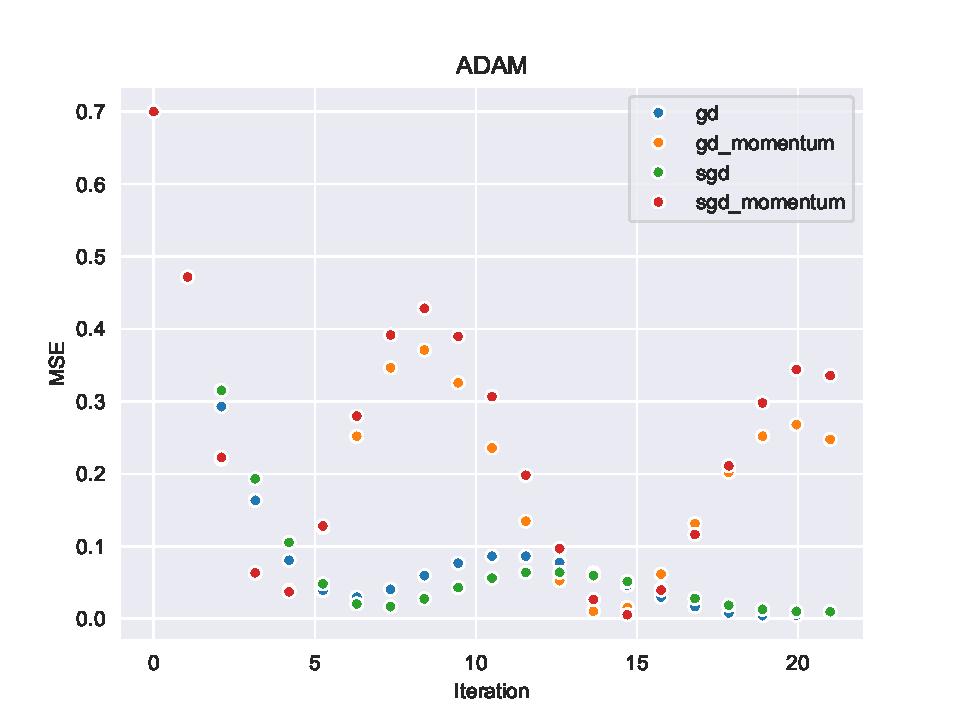
\includegraphics[width=0.8\textwidth]{Figures/PartA/ADAMMSE(iter).pdf}
\caption{MSE as a function of iterations using tuning method ADAM for plain and stochastic gradient descent with and without momentum}
\label{fig:ADAMMSE-iter-pdf}
\end{figure}


\subsection{Neural Network Regression}

\begin{figure}[htpb]
\begin{subfigure}{.5\textwidth}
  \centering
  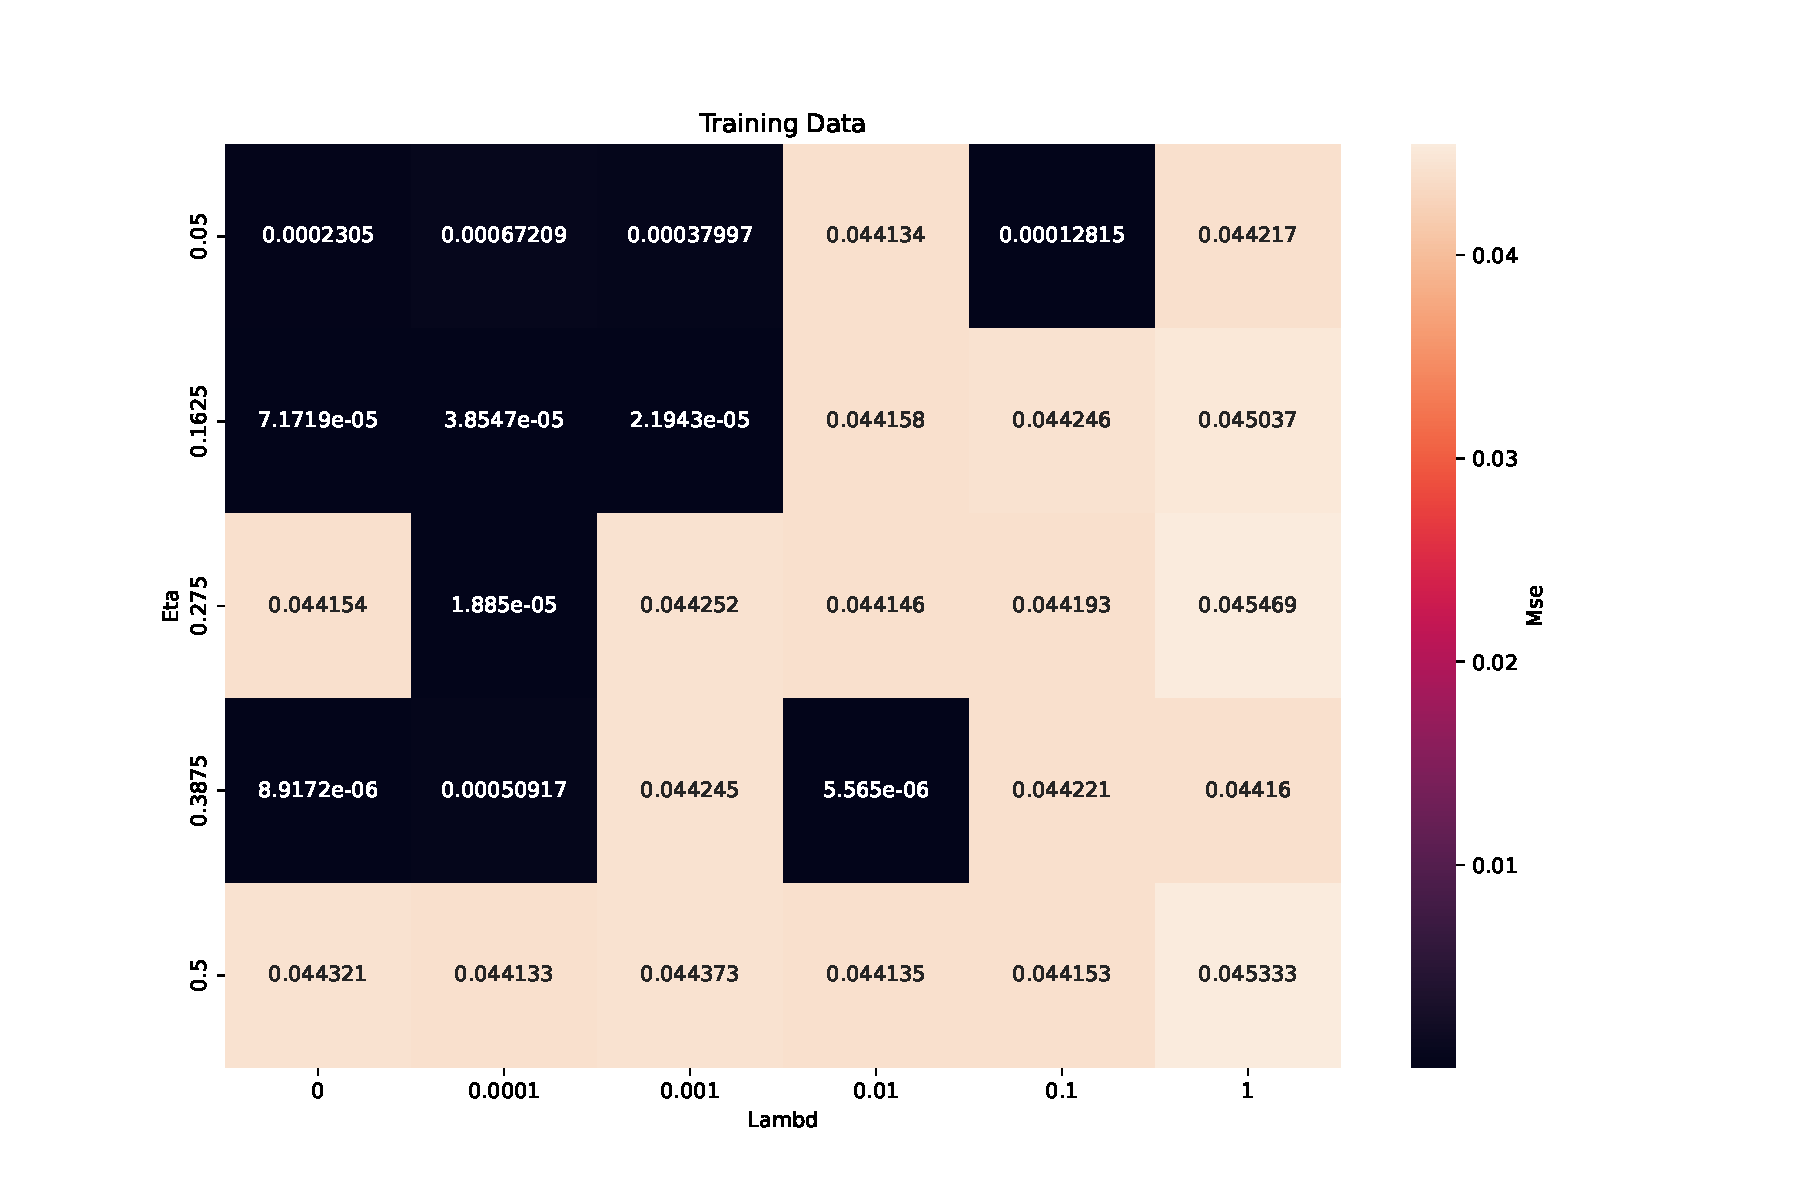
\includegraphics[width=1.2\linewidth]{Figures/PartB/train_sigmoid_MSE(eta,lmb)}
  \caption{Train MSE}
  \label{fig:train_sigmoid_MSE-eta-lmb-}
\end{subfigure}%
\begin{subfigure}{.5\textwidth}
  \centering
  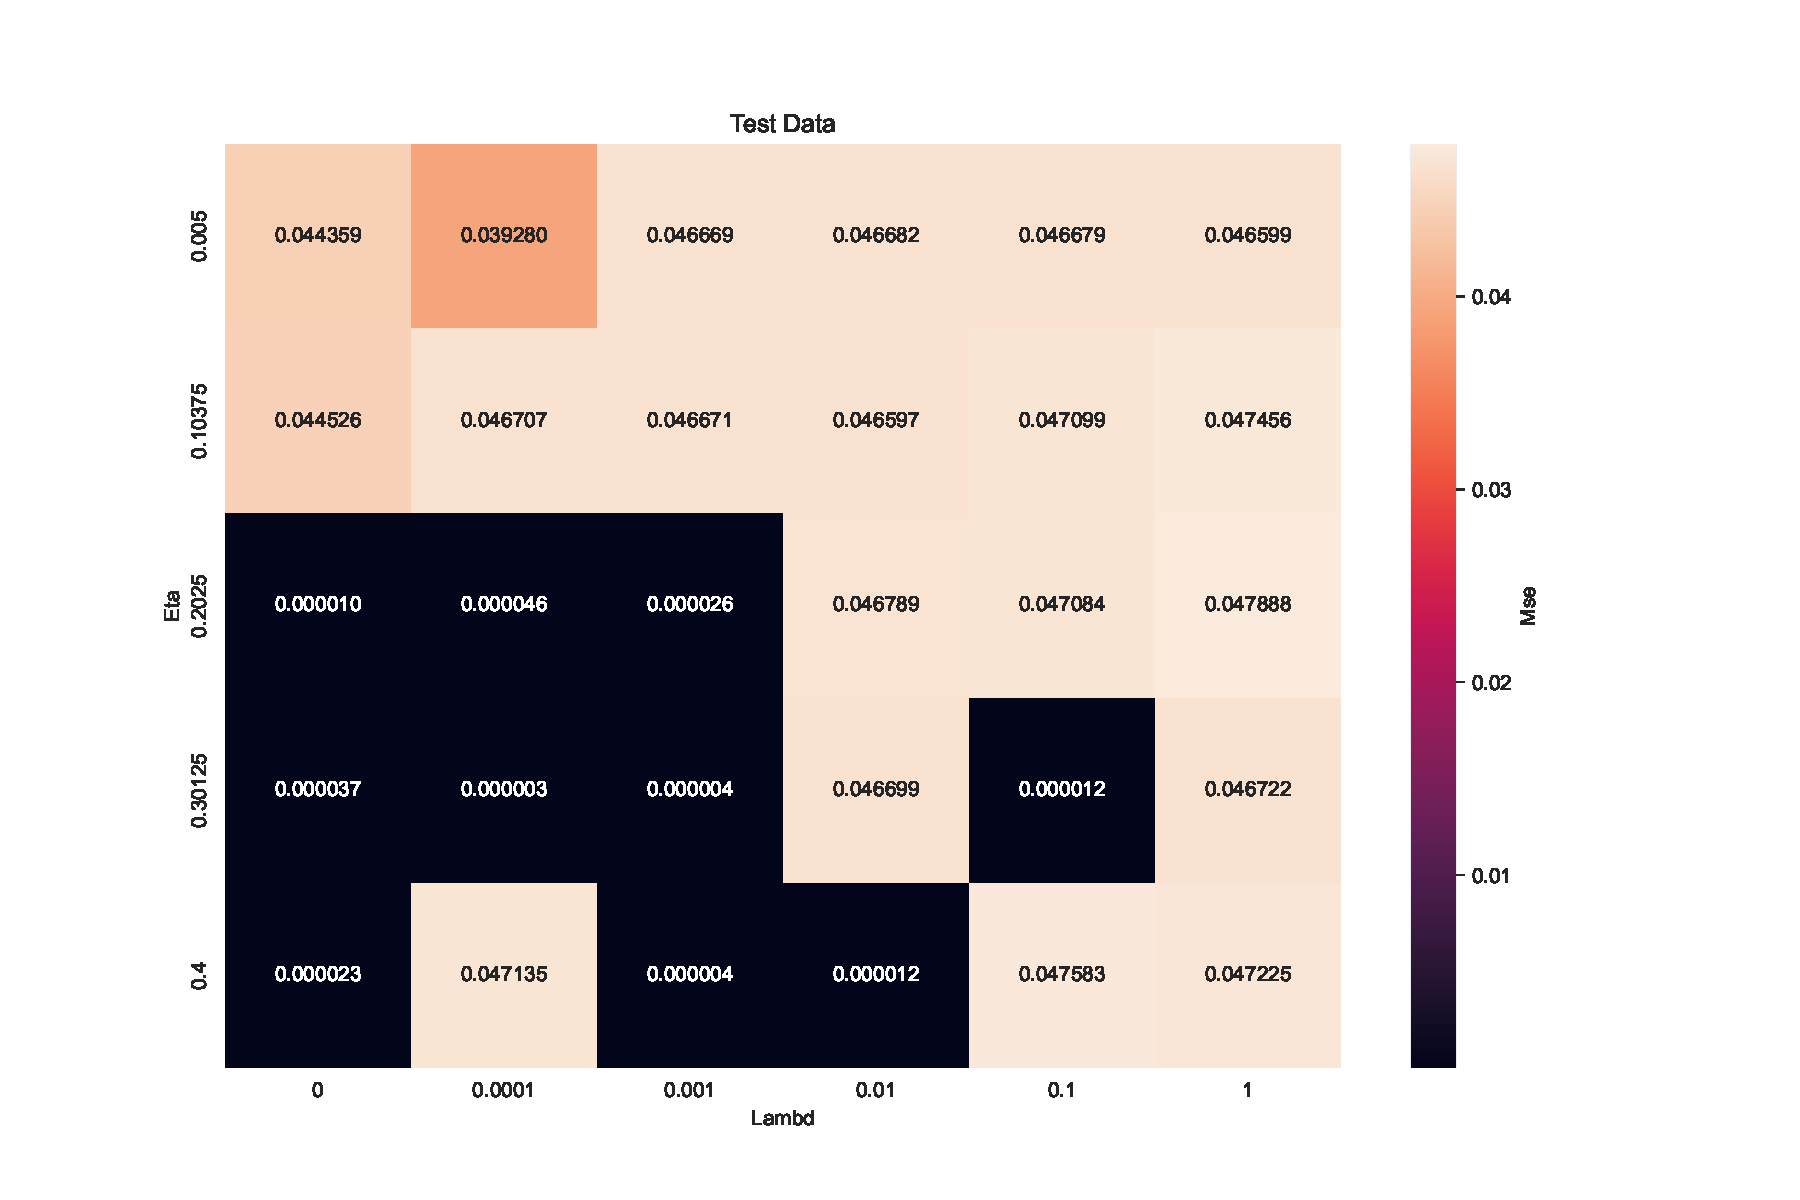
\includegraphics[width=1.2\linewidth]{Figures/PartB/test_sigmoid_MSE(eta,lmb)}
  \caption{Test MSE}
  \label{fig:test_sigmoid_MSE-eta-lmb-}
\end{subfigure}
\caption{Neural network with activation function Sigmoid MSE as a function of \(\eta \) and \(\lambda \) }
\label{fig:Sigmoid_MSE}
\end{figure}

\begin{figure}[htpb]
\begin{subfigure}{.5\textwidth}
  \centering
  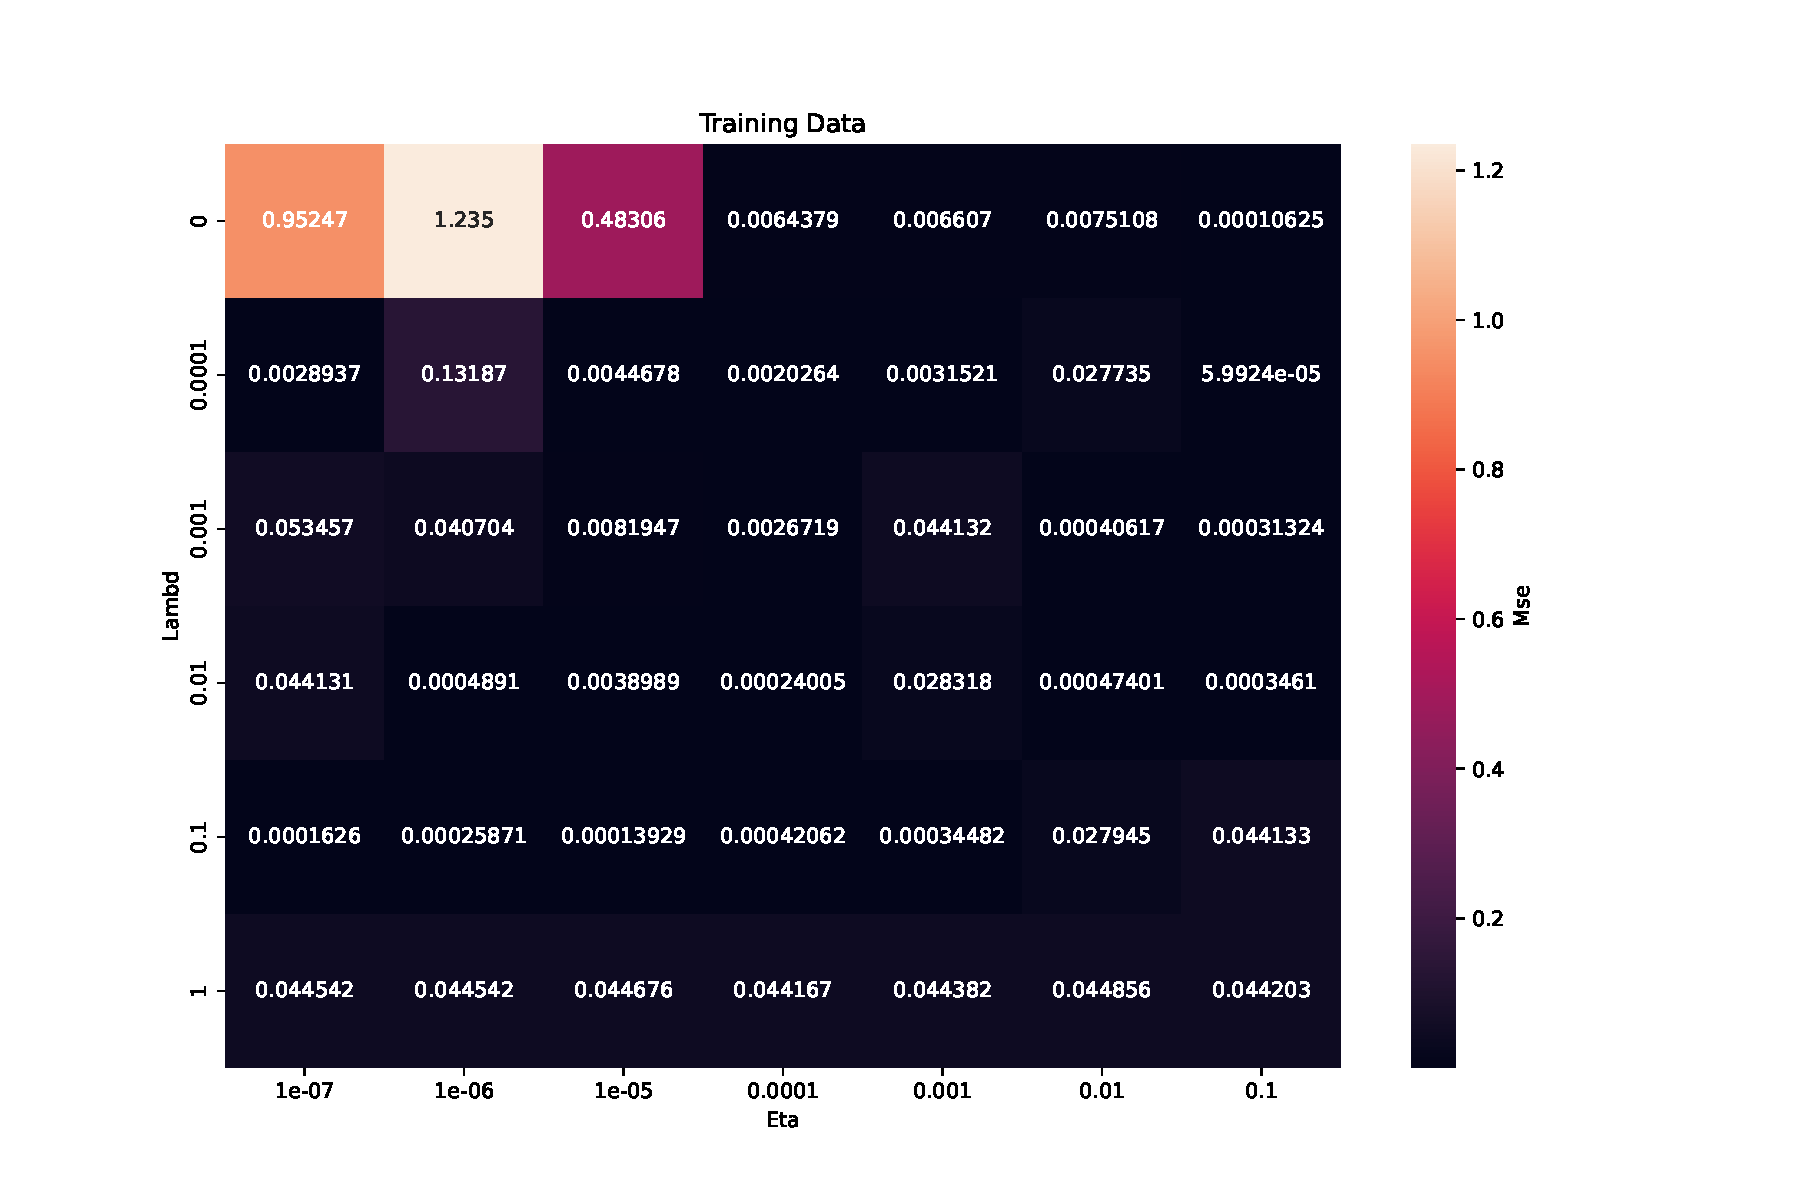
\includegraphics[width=1.2\linewidth]{Figures/PartB/train_relu_MSE(eta,lmb)}
  \caption{Train MSE}
  \label{fig:train_relu_MSE-eta-lmb-}
\end{subfigure}%
\begin{subfigure}{.5\textwidth}
  \centering
  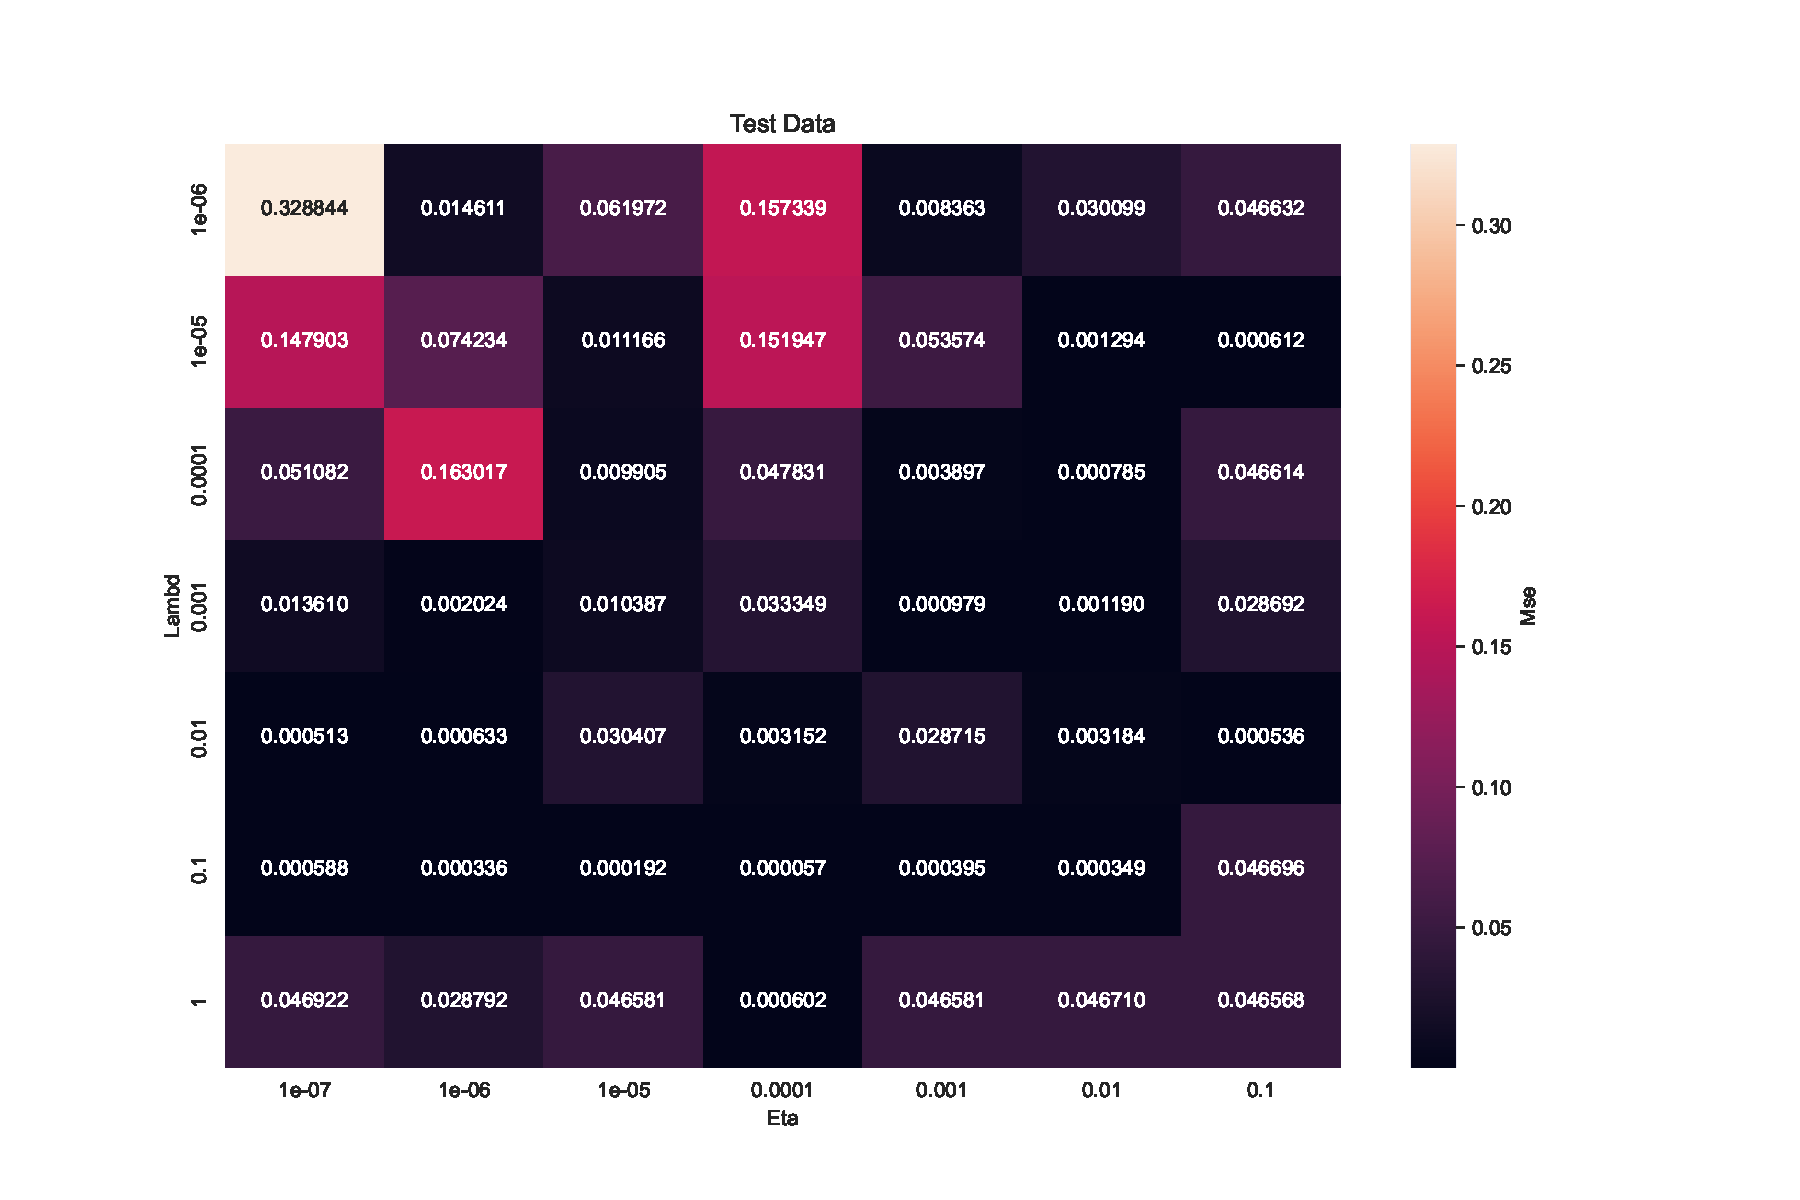
\includegraphics[width=1.2\linewidth]{Figures/PartB/test_relu_MSE(eta,lmb)}
  \caption{Test MSE}
  \label{fig:test_relu_MSE-eta-lmb-}
\end{subfigure}
\caption{Neural network with activation function relu MSE as a function of \(\eta \) and \(\lambda \) }
\label{fig:relu_MSE}
\end{figure}

\begin{figure}[htpb]
\begin{subfigure}{.5\textwidth}
  \centering
  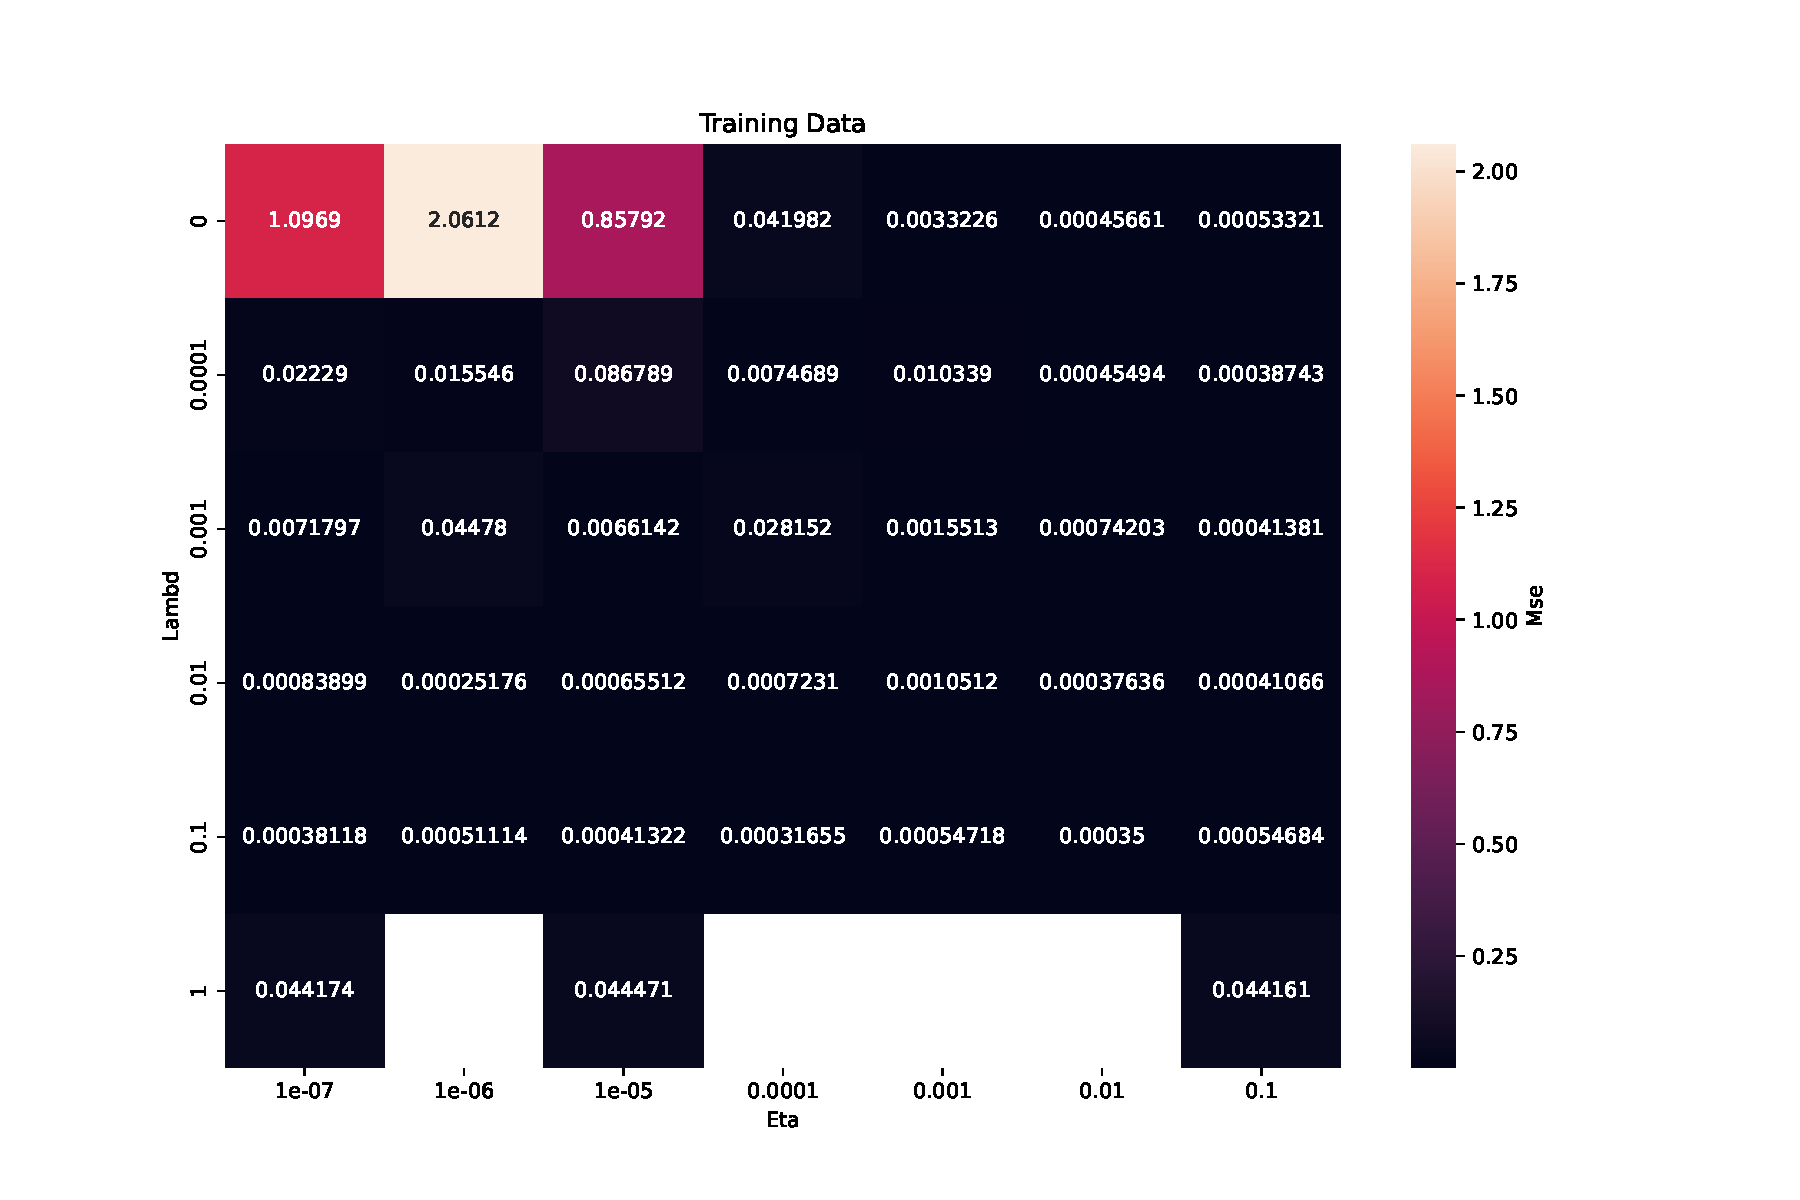
\includegraphics[width=1.2\linewidth]{Figures/PartB/train_leaky_relu_MSE(eta,lmb)}
  \caption{Train MSE}
  \label{fig:train_leaky_relu_MSE-eta-lmb-}
\end{subfigure}%
\begin{subfigure}{.5\textwidth}
  \centering
  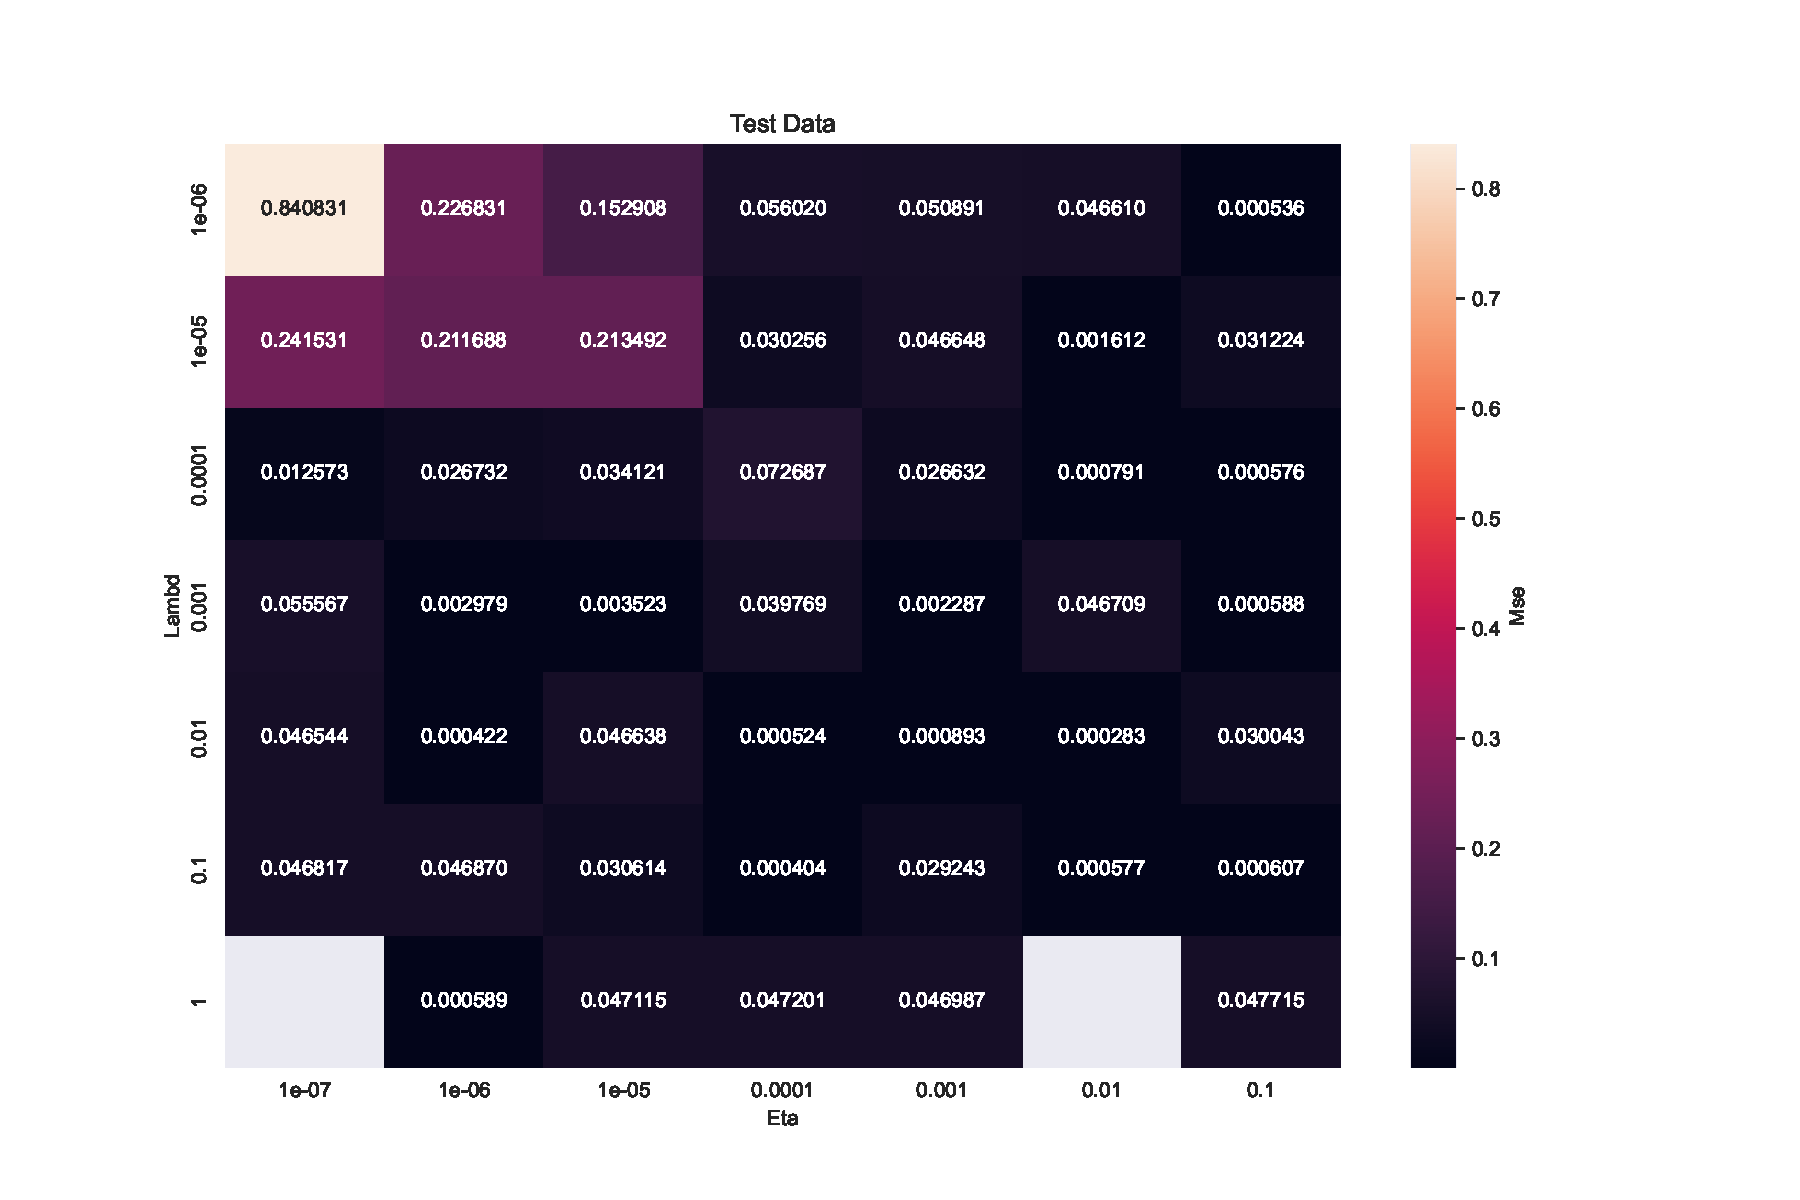
\includegraphics[width=1.2\linewidth]{Figures/PartB/test_leaky_relu_MSE(eta,lmb)}
  \caption{Test MSE}
  \label{fig:test_leaky_relu_MSE-eta-lmb-}
\end{subfigure}
\caption{Neural network with activation function leaky relu: MSE as a function of \(\eta \) and \(\lambda \) }
\label{fig:leaky_relu_MSE}
\end{figure}

\begin{figure}[htpb]
\begin{subfigure}{.5\textwidth}
  \centering
  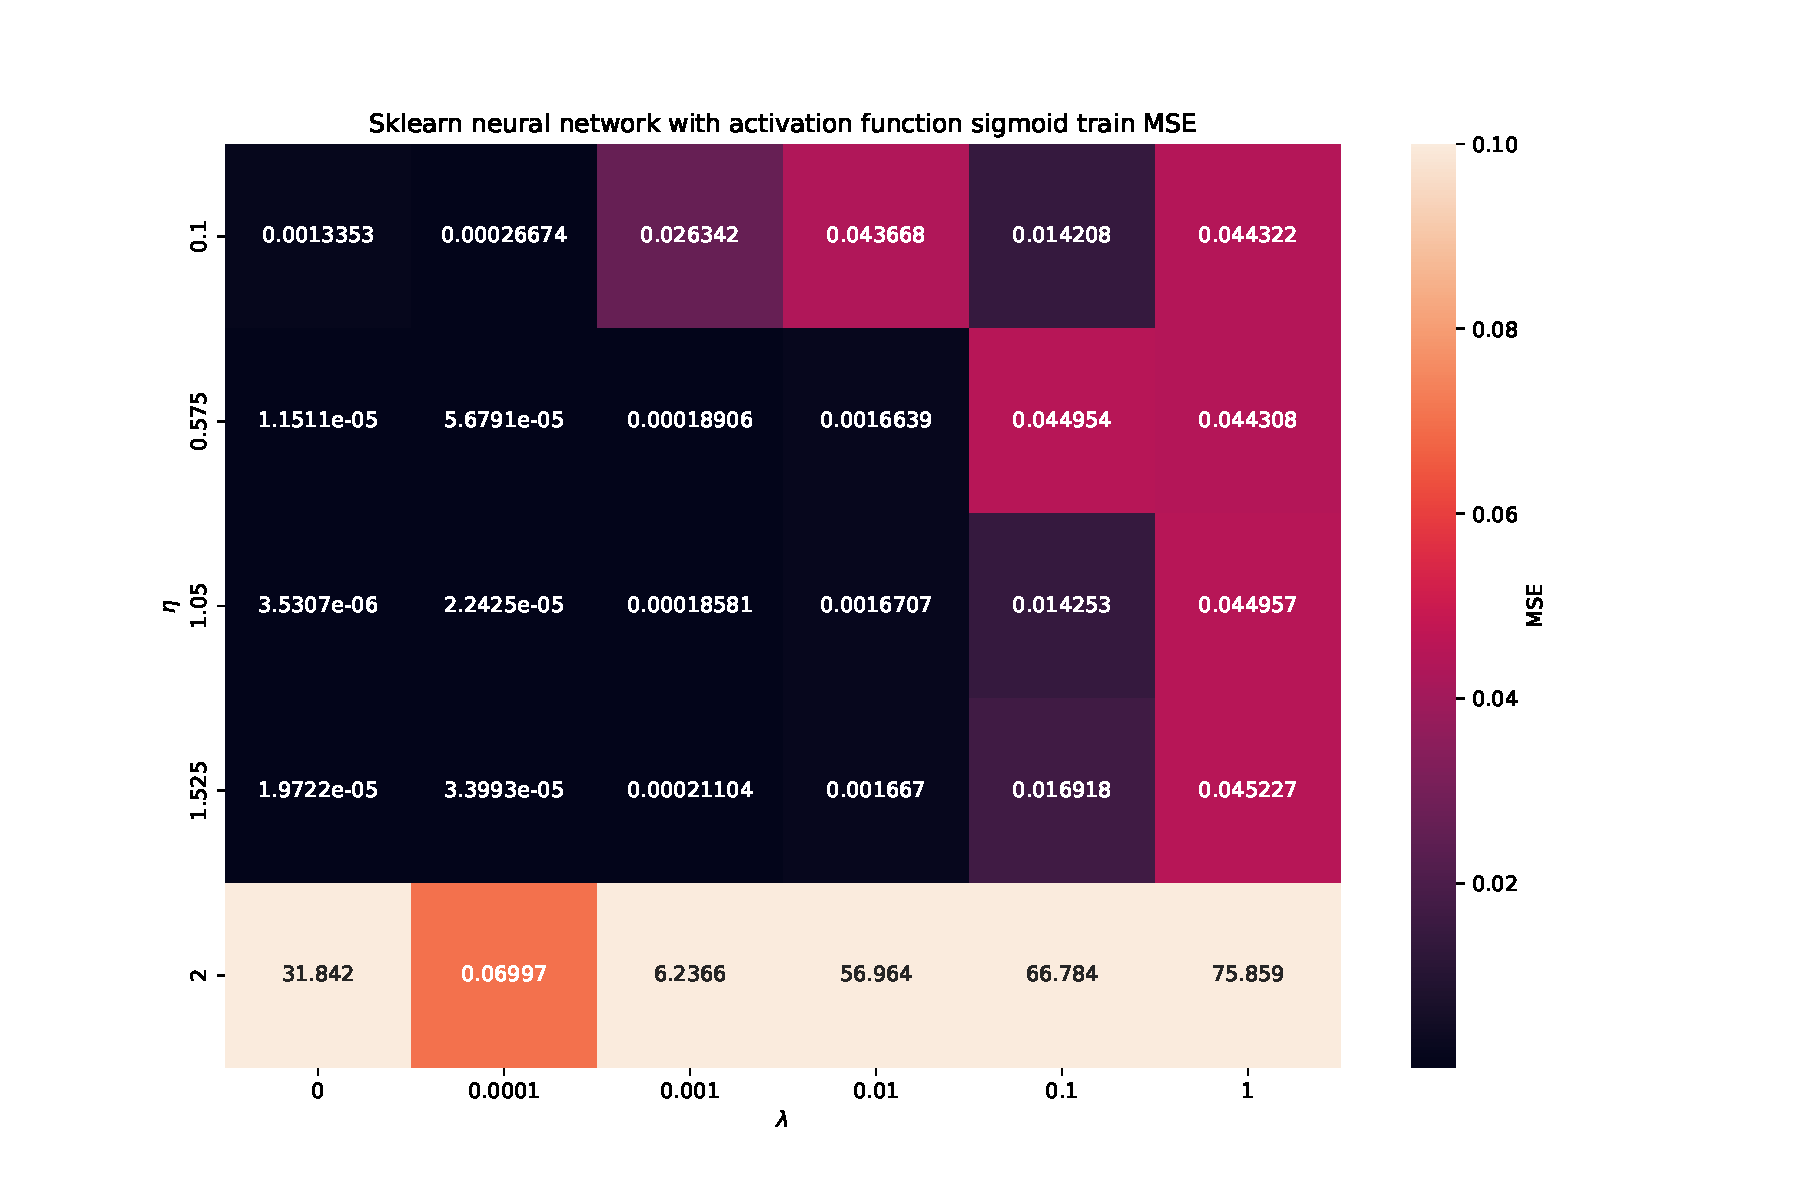
\includegraphics[width=1.2\linewidth]{Figures/PartB/train_sklearn_sigmoid_NN_MSE(eta,lmb)}
  \caption{Sigmoid MSE}
  \label{fig:train_leaky_relu_MSE-eta-lmb-}
\end{subfigure}%
\begin{subfigure}{.5\textwidth}
  \centering
  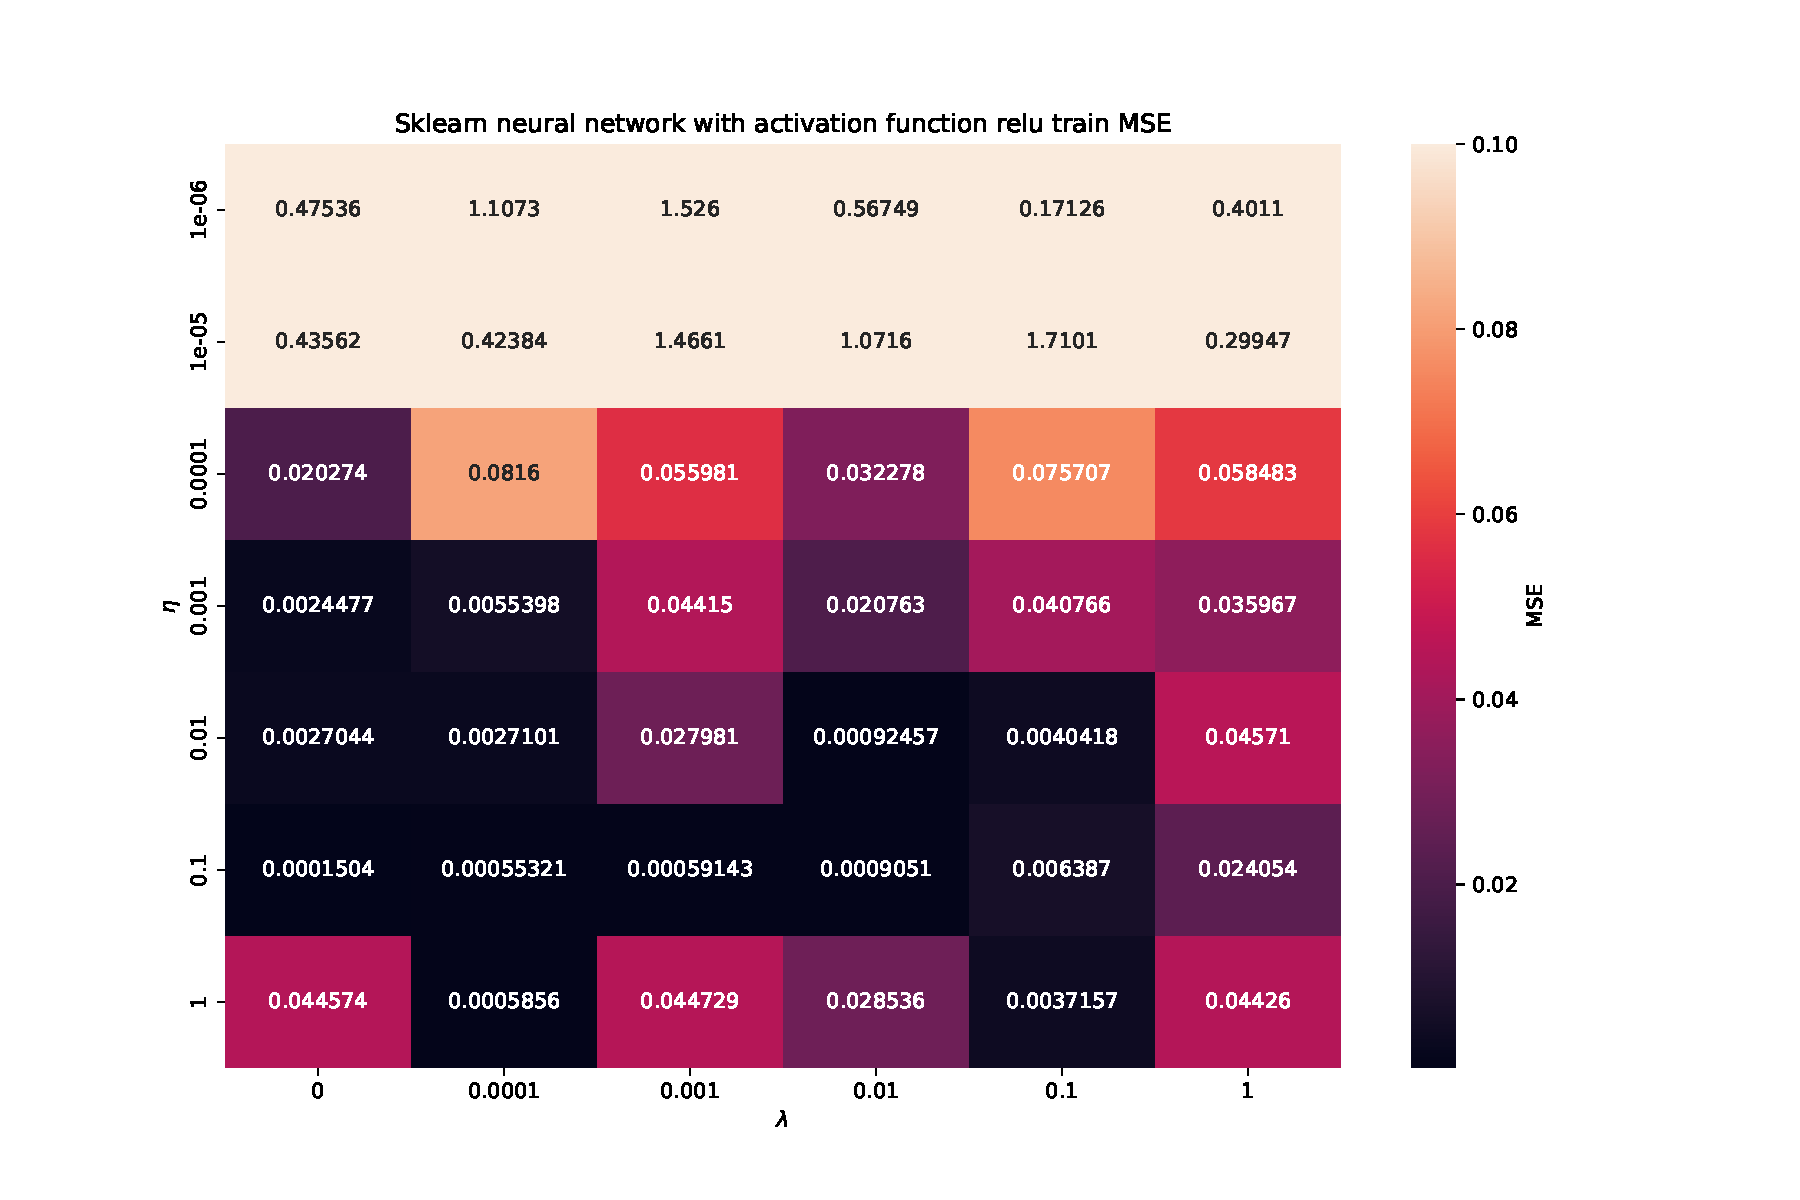
\includegraphics[width=1.2\linewidth]{Figures/PartB/train_sklearn_relu_NN_MSE(eta,lmb)}
  \caption{Relu MSE}
  \label{fig:test_leaky_relu_MSE-eta-lmb-}
\end{subfigure}
\caption{SkLearn neural network with activation function sigmoid and relu: Train MSE as a function of \(\eta \) and \(\lambda \) }
\label{fig:leaky_relu_MSE}
\end{figure}


